%\section{Arquitectura de Redundancia Propuesta RE ACOMODAR EN OTRA SECCIÓN}

%\section{Arquitectura de Redundancia Propuesta}

\section{Implementación del Sistema Tolerante a Fallas}

%\section{Sistema Tolerante a Fallas Implementado}

% En esta sección, se presenta la arquitectura implementada para la tolerancia a fallas de hardware. Como se mostró en la sección anterior, \textit{The Byzantine Generals Problem} sienta las bases para la tolerancia a fallas arbitrarias de hardware. A través de una serie de intercambios de mensajes entre los nodos de la red, estos pueden llegar a un consenso, para tomar la misma decisión. Además, se mostró que para poder tolerar una falla arbitraria, se requiere por lo menos de 4 nodos interconectados.

% Luego de presentar el problema, se hizo una comparación entre los generales leales y las computadoras de vuelo sin fallas y entre los generales traidores y las computadoras con fallas. Una de las cuestiones que no se mencionó, es el hecho de que las computadoras de vuelo constituyen sistemas de tiempo real. Esto es debido a que deben realizar tareas que requieren determinismo temporal. Por ejemplo, cálculo de la ley de control, estimación de la pose, etc... En el problema original, los generales pueden enviar sus mensajes a sus pares en cualquier momento y en cualquier orden.

% Otro de los puntos que caracterizan al problema original, es el hecho de que la comunicación entre los generales es 1 a 1. Debido a esto, los generales traidores pueden entregar información confusa a sus pares para tratar de romper el consenso. Esto es lo que vuelve complejo al problema \cite{lamport2019byzantine} y costosa a su solución \cite{roth2021not}.

% En esta sección se muestra que, si el sistema tiene ciertas características, en particular ser un sistema de tiempo real y contar con un bus común a los nodos para las comunicaciones, luego el problema del consenso se simplifica mucho.

En esta sección se presenta la arquitectura de sistema propuesta para la tarea de tolerancia a fallas. Esta consiste en un sistema distribuido, conformado por las tres computadoras de vuelo construidas para este trabajo. Se describen las características del firmware desarrollado para implementar el sistema propuesto. Para demostrar las capacidades de toleranca a fallas, se hicieron una serie de pruebas simulando fallas en un sensor. Finalmente, se muestran los resultados obtenidos sobre las pruebas realizadas.


%Para esto, se desarrolló un firmware con una arquitectura de sistema distribuido, conformado por las tres computadoras de vuelo construidas para este trabajo.

%En esta sección se presentan una serie de pruebas que demuestran las capacidades de tolerancia a fallas de la computadora de vuelo. Para ello, se desarrolló un firmware con una arquitectura de sistema distribuido, conformado por las tres computadoras de vuelo construidas para este trabajo.



%Estas consistieron en simular una serie de fallas y, a partir de la comparación entre placas, detectar las diferencias obtenidas para distintos cálculos realizados. Además, se describe el firmware desarrollado




%, por lSe utilizan tres réplicas de la computadora de vuelo

% Para implementar la tolerancia a fallas, se optó por un esquema distribuido, el cual se compone de tres unidades de la CNGC, conectadas entre sí a través del bus CAN, cada una de ellas alimentadas de manera independiente. Una imagen del stack de nodos puede observarse en la Fig. 3. Cada nodo funciona de manera independiente ejecutando exactament

%\subsection{Arquitectura Propuesta: \textit{The Time-Triggered Architecture}}
\subsection{Descripción de la Arquitectura Propuesta}

%\subsubsection{Sincronismo de los nodos}

Como fue explicado en la sección \ref{sec:disenio_computadora_de_vuelo}, la computadora de vuelo se encarga de ejecutar el sistema de navegación para guiar el vehículo en su trayectoria. Este sistema cumple con las características de ser de tiempo real, ya que tanto los valores de los resultados de cómputo, como el instante de tiempo en el que se obtienen, son de vital importancia para la correcta ejecución de las distintas tareas de control del vehículo. 
%La computadora de vuelo comprende un sistema de tiempo real. Esto quiere decir que tanto los valores de los resultados de cómputo, como el instante de tiempo en el que se obtienen, son importantes para la correcta ejecución de las distintas tareas. En la sección \ref{sec:disenio_computadora_de_vuelo}
Por otro lado, en la sección \ref{sec:requerimentos_sistema_tolerancia_fallas} se hizo un análisis de las características que deben tener este tipo de sistemas para poder implementar un mecanismo de tolerancia a fallas utilizando redundancias. A partir de lo presentado hasta aquí, las características elementales de un sistema de tiempo real con tolerancia a fallas se pueden resumir en los siguientes items:

%En la sección \ref{sec:requerimentos_sistema_tolerancia_fallas} se mencionó que se busca enmascarar fallas que puedan ocurrir, permitiendo continuar con el normal funcionamiento del sistema, a pesar de dicha falla. Para esto, el mecanismo de tolerancia a fallas consiste en el uso de redundancias y la comparación de resultados entre distintas réplicas de hardware. Además, se concluyó que la comparación de resultados se 

\begin{enumerate}
    %\item El sistema es de tiempo real, es decir, se requiere determinismo temporal en la ejecución de las tareas.
    \item Se requiere determinismo temporal en la ejecución de las tareas.
    \item La tolerancia a fallas se implementa a través de la comparación de resultados de las distintas réplicas.
    \item Para que el mecanismo de tolerancia a fallas sea efectivo, es necesario comparar resultados que se correspondan temporalmente. Esto implica que cada réplica debe ejecutar las mismas tareas en paralelo y de manera sincronizada.
    \item Es necesario utilizar un bus para el intercambio de resultados entre réplicas. A su vez, se requiere un acceso al medio por turnos, respetado por todas las réplicas.
\end{enumerate}

Una arquitectura que se ajusta a estas características corresponde a sistemas que ejecutan sus tareas en instantes de tiempo predefinidos, típicamente denominados \textit{time-triggered systems} o \textit{time-triggered architecture}. La característica principal es que presentan un fuerte determinismo temporal, ya que el instante de tiempo en el que se ejecuta cada tarea se vuelve parte del diseño del sistema. Esta característica facilita su uso en sistemas críticos de tiempo real, debido a que su comportamiento es predecible \cite[p.~12]{pont2008patterns}. Pueden encontrarse trabajos \cite{kopetz2003time} \cite{kopetz1998time} y libros \cite{kopetz-2011} \cite{pont2008patterns} que explican formalmente esta arquitectura y sus distintos componentes con más detalle. En esta sección se pretende describir brevemente sus características más relevantes.


%A continuación, se presenta brevemente los componentes y el funcionamiento de la arquitectura para el sistema de este trabajo.

% =================================================
% Explicación breve de time triggered systems:
% Set de tareas periódicas que se ejecutan en instantes de tiempo predefinidos. Estas tareas son run-to-completion.
% Existe un scheduler que se ejecuta en cada réplica, el cual determina cuál es la siguiente tarea a ejecutar. Ese scheduler está controlado por el paso del tiempo, típicamente por la interrupción de un timer. Esta es la única interrupción que se permite en el sistema. El scheduler es cooperative.
% Las comunicaciones también se incluyen en el scheduling, tanto el envío de mensajes como la recepción. No se permiten las retransmisiones, a menos que sean parte del scheduling predefinido.
% Debido a que el scheduling es predefinido y se sabe cuándo se debería ejecutar cada tarea, en el eventual caso en el que una tarea no pueda ser ejecutada a tiempo, esto es fácilmente dectable y puede tomarse una acción correctiva.

% El aspecto restante es el de la sincronización, necesaria para ejecutar la tolerancia a fallas adecuadamente. Las características del sistema con scheduler predefinido se prestan a la implementación de la sincronización. Al ejecutar una sincronización de los timers de los schedulers de cada réplica, se está sincronizando la ejecución de las tareas.

% Con todo esto, se puede enmascarar 1 sola falla simultánea, de cualquiera de las 3 réplicas, en el sistema total.

En la figura \ref{fig:esquema_time_triggered_architecture} se muestra un esquema que se corresponde con del funcionamiento de un sistema \textit{time-triggered}, donde se ilustra una simplificación del funcionamiento de la computadora de vuelo. En el instante de tiempo $t_1$ se obtienen mediciones de acelerómetros y giróscopos, en el instante $t_2$ se ejecuta el algoritmo de navegación y en $t_3$ se aplica un nuevo comando sobre los actuadores del vehículo.

%{\Large \textbf{{\color{red} PONER LA IMAGEN DEL SCHEDULER CON EL SET DE TAREAS Y LOS INSTANTES DE TIEMPO PREDEFINIDOS. ESTA IMAGEN TIENE QUE TENER UN RELOJITO QUE EXPLICITE QUE LAS TAREAS SE EJECUTAN GRACIAS AL CLOCK}}}

\begin{figure}[H]
    \centering
    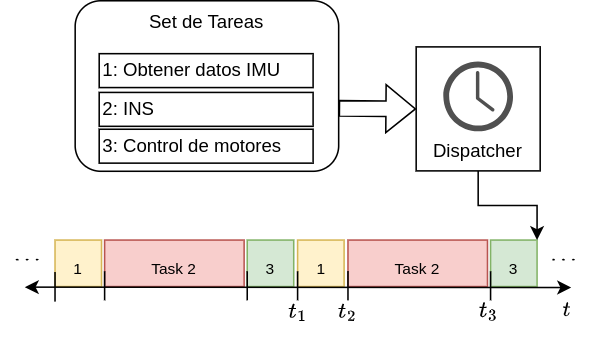
\includegraphics[width=0.7\textwidth]{img/esquema_time_triggered_architecture.png}
    \caption{Esquema del sistema time-triggered. Dentro de las especificaciones de cada tarea se encuentran sus características temporales. Estas son utilizadas por un dispatcher, para saber en qué momento deben ser ejecutadas. Para el ejemplo de esta imagen, la secuencia de ejecución es periódica. Primero se obtienen datos del sensor IMU. Estos datos se utilizan en la tarea 2 para ejecutar algoritmos de estimación y control del vehículo. Finalmente, la nueva señal de control calculada en la tarea 2, se aplica a los motores en la tarea 3. El ciclo se repite periódicamente.}
    \label{fig:esquema_time_triggered_architecture}
\end{figure}

%Este comportamiento se diferencia de sistemas  con respuesta a eventos.

La gran mayoría de sistemas embebidos emplean mecanismos que trabajan a partir de ejecutar una respuesta frente a eventos, como por ejemplo a través del uso de interrupciones. Los periféricos de un microcontrolador cuentan con mecanismos para informar al procesador de la ocurrencia de determinado evento, como por ejemplo la recepción de un nuevo byte en una interfaz UART, o el cambio de nivel en una entrada de propósito general GPIO. El hecho de que estos eventos puedan ocurrir en cualquier momento y en cualquier orden, puede comprometer el determinismo temporal. 

Un caso común es el de los sensores MEMS, los cuales suelen integrar un mecanismo para avisar al microcontrolador que hay nuevos datos de acelerómetros y giróscopos disponibles, a traveś de uno de sus terminales. Este se puede conectar a un GPIO del microcontrolador y configurar una interrupción por flanco ascendente. El set de tareas de la figura \ref{fig:esquema_time_triggered_architecture} puede estructurarse para incluir esta interrupción, como se muestra en la figura \ref{fig:esquema_event_triggered_architecture}. En este ejemplo puede verse que la tarea de control de motores se retrasa debido a esta interrupción. En el caso time-triggered, el orden e instantes de tiempo de ejecución se vuelven parte del diseño del sistema, evitando que las tareas se retrasen y puedan cumplir con su timing.

%De manera de ilustrar esto, se presenta un ejemplo en la figura . Para el primer caso, la ocurrencia de las interrupciones genera que la tarea main retrase su ejecución. Por el contrario, para el caso \textit{time-triggered}, el orden e instantes de tiempo de ejecución se vuelven parte del diseño del sistema, permitiendo que la tarea main se complete sin ser interrumpida, logrando cumplir con su timing.

\begin{figure}[H]
    \centering
    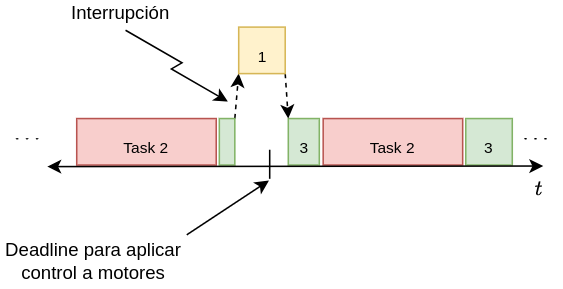
\includegraphics[width=0.7\textwidth]{img/esquema_event_triggered_architecture.png}
    \caption{Mismo set de tareas que en la figura \ref{fig:esquema_time_triggered_architecture}, pero con una arquitectura event-triggered. La interrupción genera que se ejecute la tarea 1. Debido a que las interrupciones pueden ocurrir en cualquier momento, se puede ver afectado el timing del sistema. Teniendo en cuenta que se trata de un sistema de tiempo real, esto no es aceptable y debe tratarse de una forma controlada, por ejemplo a través de una arquitectura time-triggered.}
    \label{fig:esquema_event_triggered_architecture}
\end{figure}

%{\Large \textbf{{\color{red} PONER LA IMAGEN TIPO LA DEL LIBRO DE PONT, DE LA SECCIÓN 1.7}}}

%En la figura  se considera un ejemplo muy sencillo donde ocurren 2 eventos casi de manera simultánea. A diferencia de esto, en un sistema \textit{time-triggered} las tareas del sistema no pueden ejecutarse en cualquier momento. En la figura se muestra una comparación entre ambos casos. En un sistema \textit{event-triggered}


%Este comportamiento se diferencia de sistemas con respuesta a eventos, como puede ser una interfaz con una persona, donde el usuario puede interactuar con esta para obtener una respuesta asociada casi inmediata. Este tipo de sistemas se llaman \textit{event-triggered} y son controlados por los eventos que puedan ocurrir en su entorno. A priori, se asumen eventos asincrónicos, es decir, que pueden ocurrir en cualquier momento y en cualquier orden. A diferencia de esto, en un sistema \textit{time-triggered} las tareas del sistema no pueden ejecutarse en cualquier momento. En la figura se muestra una comparación entre ambos casos. En un sistema \textit{event-triggered}

Muchos sistemas controlados por eventos funcionan con sistemas operativos de tiempo real, los cuales disponen de un scheduler que elige cuál es la tarea que corresponde ejecutar. Este aspecto también es una característica de los sistemas \textit{time-triggered}, aunque la diferencia se encuentra en la estrategia utilizada. En el caso de un RTOS es común el uso de \textit{schedulers} expropiativos con un sistema de prioridades. En un sistema \textit{time-triggered}, el \textit{scheduler} utiliza un reloj, típicamente implementado con un periférico timer, el cual determina cuál es la tarea a ejecutar. Además, a diferencia de algunos RTOS, no se utiliza el cambio de contexto, sino que cada tarea que se ejecuta, retorna y devuelve el control al \textit{scheduler} para ejecutar la siguiente tarea. Estos aspectos refuerzan el determinismo del sistema, lo que se traduce en un comportamiento predecible y por ende seguro \cite[p.~247]{pont2008patterns}.

%los schedulers pueden ser \textit{preemptive} o bien cooperativos. La ventaja de utilizar un scheduler cooperativo es nuevamente el determinismo en la ejecución de las tareas \cite[p.~247]{pont2008patterns}. Que el \textit{scheduler} sea cooperativo quiere decir que cada tarea cede el control del procesador a la siguiente tarea. Esto se implementa con tareas que se ejecutan y retornan, es decir, no se utilizan métodos como el cambio de contexto, típico de RTOS como FreeRTOS. Nuevamente, el motivo de esta decisión es darle determinismo al sistema. 



% HABLAR DE QUE LA COMUNICACIÓN SE IMPLEMENTA COMO UNA TAREA MÁS EN EL SCHEDULER

% Las comunicaciones también se incluyen en el scheduling, tanto el envío de mensajes como la recepción. No se permiten las retransmisiones, a menos que sean parte del scheduling predefinido.

En cuanto a la comparación de resultados entre distintas réplicas, estas realizarán la comparación de resultados a través de un bus de comunicaciones. %Este es el medio a través del cual los nodos intercambian información. Como se describió anteriormente, la arquitectura requiere la sincronización de los nodos para una ejecución consistente. Esto quiere decir que como mínimo, los nodos intercambian mensajes utilizados para la sincronización entre estos. Más allá de esto, en un sistema distribuido, lo más común es que haya un intercambio de información constante entre nodos.
De manera de minimizar las colisiones y favorecer el cumplimiento en el timing del sistema de tiempo real, el envío y recepción de los mensajes se implementa por turnos. La arquitectura que se utiliza facilita la implementación de este mecanismo, por ejemplo a partir del uso de tareas que estén dedicadas a recibir o enviar un mensaje a través del bus. %Esto corresponde a un protocolo de acceso al medio denominado \textit{Time Division Multiple Access} (TDMA).
En la figura \ref{fig:TDMA_esquema} se muestra un caso para 3 réplicas. Este gráfico tiene una similitud con el gráfico de la figura \ref{fig:esquema_time_triggered_architecture}. Mientras la réplica 1 ejecuta su tarea para enviar un mensaje, las réplicas 2 y 3 ejecutan una tarea para recibir ese mensaje. 

\begin{figure}[H]
    \centering
    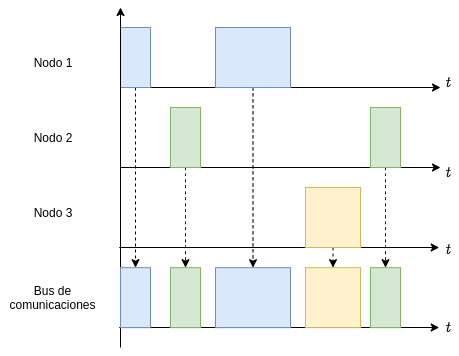
\includegraphics[width=0.6\textwidth]{img/TDMA_esquema.png}
    \caption{El ejemplo muestra como las 3 réplicas pueden compartir el bus de comuncaciones. Cada una de ellas sabe en qué instante de tiempo enviar un mensaje y en qué instantes de tiempo recibirán un mensaje. Para que esto funcione adecuadamente, las réplicas deben estar sincronizados.}
    \label{fig:TDMA_esquema}
\end{figure}

%\textbf{{\color{red} ACÁ MENCIONAR ALGUNOS PROTOCOLOS COMO FLEXRAY O TTP/C QUE DE POR SÍ YA EJECUTAN UNA SINCRONIZACIÓN.}}

%En \cite{kopetz2003time} se define un elemento del nodo denominado \textit{Communication Network Interface}(CNI). Esta es una interfaz entre el software del nodo y el acceso al medio físico. Utilizando el protocolo de acceso al medio TDMA, el software del nodo \textit{pushea} un mensaje a la CNI. Es esta última la que se encarga de administrar los tiempos de envío y recepción. Es decir, mientras el nodo continua con sus tareas, la CNI se encarga de cumplir con el timing del envío del mensaje.

% \begin{figure}[H]
%     \centering
%     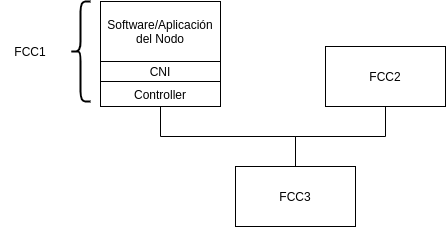
\includegraphics[width=0.6\textwidth]{img/TTA_Bus.png}
%     \caption{Misma imagen que \ref{fig:byzantine_bus_2}. Se muestra el detalle de los nodos, en el nodo FCC1.}
%     \label{fig:TTA_Bus}
% \end{figure}

%Al recibir un mensaje, ocurre algo similar. El software del nodo \textit{pollea} a la CNI en determinado instante de tiempo para obtener el mensaje recibido. Otra forma de implementar esto podría ser a través de una interrupción en el software, es decir, que cuando llege un mensaje nuevo, se dispare una interrupción en el software. El problema con esto es que se le quita determinismo al sistema.



% Debido a que el scheduling es predefinido y se sabe cuándo se debería ejecutar cada tarea, en el eventual caso en el que una tarea no pueda ser ejecutada a tiempo, esto es fácilmente dectable y puede tomarse una acción correctiva.

El hecho de que el comportamiento del sistema sea predecible facilita la tarea de detección del fracaso del cumplimiento del scheduling de las tareas. Esto puede hacerse en tiempo de ejecución. En la figura \ref{fig:task_overrun} se muestra un ejemplo donde una tarea excede su tiempo de ejecución normal. Si esto no es monitoreado adecuadamente, podría bloquearse la ejecución de la siguiente tarea. Debido a que se conoce qué tarea se está ejecutando y cuál debería ejecutarse, fácilmente puede detectarse el fracaso en la ejecución y tomar una acción en consecuencia.

%{\Large \textbf{{\color{red} IMAGEN CON UN TASK OVERRUN}}}

\begin{figure}[H]
    \centering
    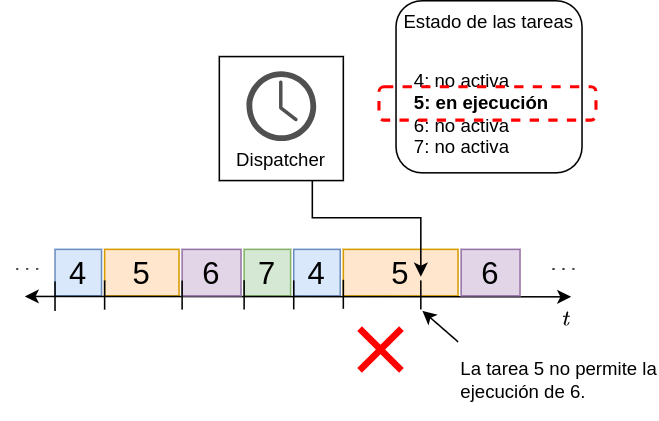
\includegraphics[width=0.6\textwidth]{img/task_overrun.png}
    \caption{La tarea 5 bloquea la ejecución de la 6, evitando que se cumpla el scheduling. Mientras se ejecuta la tarea 5, se llama al dispatcher para ejecutar la siguiente, tarea 6. Gracias a que el dispatcher conoce el estado de las tareas, este detecta que la tarea 5 no ha finalizado su ejecución y por ende que no se ha respetado el scheduling.}
    \label{fig:task_overrun}
\end{figure}


% El aspecto restante es el de la sincronización, necesaria para ejecutar la tolerancia a fallas adecuadamente. Las características del sistema con scheduler predefinido se prestan a la implementación de la sincronización. Al ejecutar una sincronización de los timers de los schedulers de cada réplica, se está sincronizando la ejecución de las tareas.

% Con todo esto, se puede enmascarar 1 sola falla simultánea, de cualquiera de las 3 réplicas, en el sistema total.

% Puntapié para hablar de la sincronización
Para que no haya colisiones en el bus de comunicaciones, todas las réplicas deben respetar el timing, el cual se encuentra predefinido gracias al \textit{scheduler}. Sumado a esto, para que las comparaciones de resultados permitan la detección de fallas, los valores a comparar deben corresponderse temporalmente. Ambas cuestiones se resuelven a partir de la sincronización de los \textit{schedulers} de cada una de las réplicas, la cuál debe ejecutarse de forma periódica.

El comportamiento de cada una de las réplicas está controlado en última instancia por el \textit{timer} del \textit{scheduler}. Por más que todas las réplicas presenten circuitos osciladores exactamente iguales y de la misma frecuencia, inevitablemente existirá un efecto de \textit{drift}, ya sea por cuestiones mismas de fabricación o por efecto de la temperatura. Esto traerá como consecuencia que los \textit{timers} y por ende los \textit{schedulers} se desfasen a medida que pasa el tiempo. 
%Este efecto puede verse en la figura  . En el instante inicial, los \textit{schedulers} se encuentran sincronizados, pero debido a las diferencias en los osciladores de cada réplica, al cabo de un tiempo, el sistema perderá el sincronismo y fracasará.

%{\Large \textbf{{\color{red} IMAGEN CON DESINCRONISMO}}}

Para solucionar este problema, se requiere la ejecución de una resincronización periódica. El desfasaje entre los clocks de cada réplica irá creciendo conforme pase el tiempo. En la figura \ref{fig:esquema_desincronizacion} se muestra un ejemplo donde cada réplica tiene un drift $\rho$ distinto. Una forma de corrección puede ser como la que se muestra en la figura \ref{fig:esquema_resincronizacion}. Al corregir el offset entre clocks periódicamente puede controlarse el desfasaje, manteniéndolo en niveles aceptables. Las réplicas quedarán sincronizados con cierta precisión $\Pi$. Existen muchísimos algoritmos de resincronización, en \cite{anceaume1998performance} se puede encontrar un estudio que compara distintos tipos de algoritmos. En \cite{9501400} puede encontrarse un trabajo donde se implementa una sincronización entre distintos miembros de un bus CAN, donde no solo se hace una corrección del desfasaje, sino que además se corrige la velocidad de cada clock, obteniendo una precisión inferior a 1 $\mu$s.

% \begin{figure}[H]
%     \centering
%     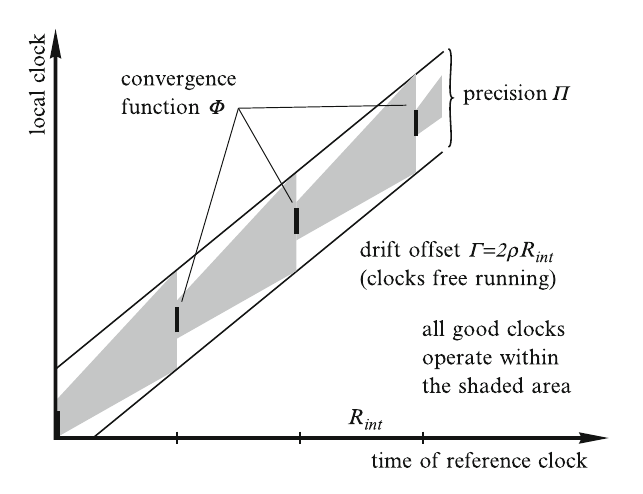
\includegraphics[width=0.7\textwidth]{img/TTA_resincronizacion.png}
%     \caption{El eje horizontal representa el paso del tiempo físico y el eje vertical el avance de cada clock local a cada nodo. El valor $R_{int}$ corresponde al período de resincronización. La imagen se extrajo de \cite[p.~67]{kopetz-2011}.{\color{red} ACÁ PONER UNA IMAGEN HECHA POR MÍ} }
%     \label{fig:TTA_resincronizacion}
% \end{figure}

\begin{figure}[H]
    \centering
    \begin{subfigure}[b]{0.48\textwidth}
        \centering
        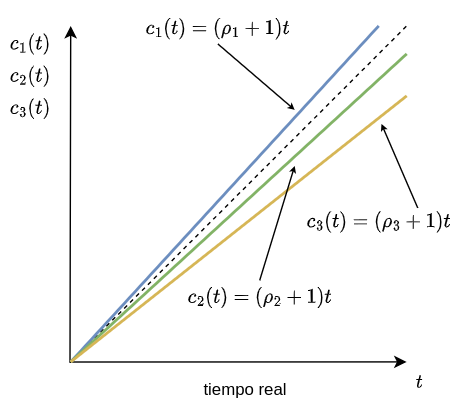
\includegraphics[width=\textwidth]{img/esquema_desincronizacion.png}
        \caption{Caso sin sincronización, las réplicas se desfasan, impidiendo la correcta ejecución del sistema.}
        \label{fig:esquema_desincronizacion}
    \end{subfigure}
    %\hfill
    \begin{subfigure}[b]{0.48\textwidth}
        \centering
        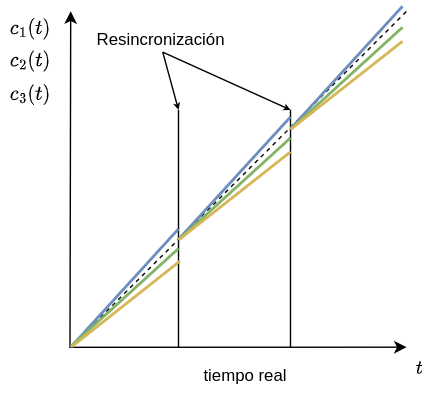
\includegraphics[width=\textwidth]{img/esquema_resincronizacion.png}
        \caption{La resincronización periódica mantiene el desfasaje en valores controlados.}
        \label{fig:esquema_resincronizacion}
    \end{subfigure}
       \caption{Se muestra cómo el efecto de la resincronización periódica evita el desfasaje entre réplicas. En el eje horizontal se ubica el paso del tiempo real, mientras que el eje vertical corresponde a los clocks de las 3 réplicas, $c_1(t)$, $c_2(t)$ y $c_3(t)$. En línea punteada se muestra el caso de un clock perfecto sin drift.}
       \label{fig:esquema_desinc_resinc}
\end{figure}

%De forma de que el funcionamiento del sistema de tiempo real distribuido sea correcto, todos los nodos deben ejecutar sus tareas de forma consistente. Para ello, sus schedulers deben estar sincronizados. Para el caso de este trabajo, cada una de las FCCs debe encontrarse ejecutando la misma tarea al mismo tiempo. De esta forma pueden ejecutarse los algoritmos de votación para realizar tolerancia a fallas de hardware, como ya se describió anteriormente.

Algunos sistemas distribuidos de tiempo real utilizan un clock maestro, implementado como un miembro del sistema, al que todas las demás réplicas utilizan como referencia. Por ejemplo, la extensión del protocolo automotivo CAN, denominada Time-Triggered CAN (TTCAN) \cite{leen2002ttcan} utiliza esta estrategia. La desventaja de este método es que dicho clock maestro se convierte en un punto singular de falla: si este presenta una falla, habrá un error en la sincronización, lo que decantará en el fracaso de todo el sistema.

Otra forma es utilizar una base de tiempos global \cite[p.~51]{kopetz-2011}. Esta se define como un acuerdo entre las réplicas respecto a una base de tiempo común que será utilizada como referencia. Por ejemplo, las 3 réplicas pueden intercambiar valores de sus clocks, obtener un promedio y corregir sus desfasajes contra ese valor, evitando el uso de un clock maestro. %Esta puede implementarse por ejemplo utilizando un contador local. 
%Idealmente, para que las réplicas puedan utilizar este contador como base de tiempos, todas ellas deben tener el mismo valor, al mismo tiempo. En la práctica esto no es posible, por el efecto del \textit{drift} mencionado anteriormente y luego existirá cierta precisión en la sincronización, la cual dependerá del hardware y del algoritmo utilizado.
%En la práctica este acuerdo esto no es posible, por el efecto del \textit{drift} mencionado anteriormente y luego existirá cierta precisión en la sincronización, la cual dependerá del hardware y del algoritmo utilizado.

Tomando todas los aspectos mencionados hasta aquí, el funcionamiento del sistema distribuido puede ilustrarse como en la figura \ref{fig:diagrama_TTA}. Cada una de las réplicas ejecuta una serie de tareas de forma periódica con cierto \textit{timing} definido. Además, existe una base de tiempos común a todas las réplicas, permitiendo la ejecución coordinada y sincronizada. Debido a que la sincronización debe ejecutarse de forma periódica y aprovechando las características del \textit{scheduler}, la implementación de la tarea que corrija el desfasaje de cada clock puede incluirse como una tarea dentro del \textit{scheduling}.


\begin{figure}[H]
    \centering
    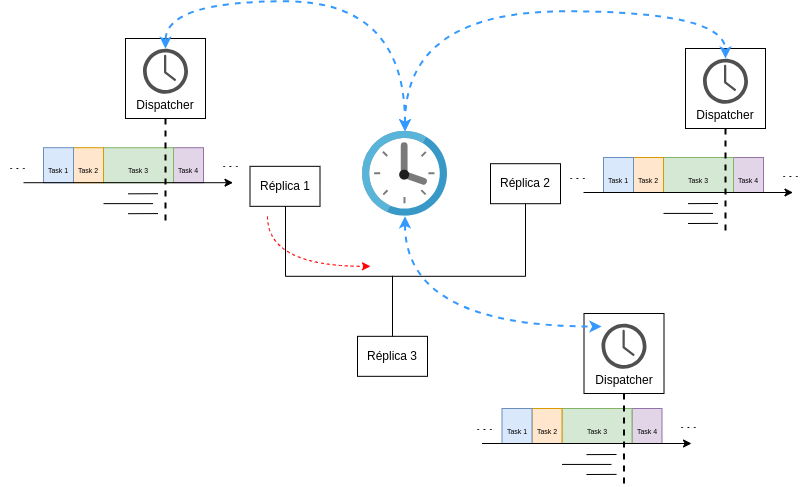
\includegraphics[width=\textwidth]{img/diagrama_TTA.png}
    \caption{Se muestra un esquema que representa la arquitectura. Cada réplica tiene un \textit{clock} local, funcionando a partir de su propio cristal. Todos estos a su vez se sincronizan periódicamente, representado por el reloj azul en el centro. En la imagen, la réplica 1 se encuentra enviando un mensaje por el bus. Al mismo tiempo, las réplicas 2 y 3 ejecutan una tarea que corresponde a recibir un mensaje y almacenarlo en memoria.}
    \label{fig:diagrama_TTA}
\end{figure}



% Con todo esto, se puede enmascarar 1 sola falla simultánea, de cualquiera de las 3 réplicas, en el sistema total.

%Una forma de realizar la corrección del \textit{timer} es sobreescribiendo su valor con un nuevo valor calculado a partir del algoritmo de sincronización. Este método puede generar inconsistencias en la ejecución de las tareas del nodo \cite[p.~72]{kopetz-2011}. La forma que se prefiere es ir aplicando correcciones sucesivas conforme se van reajustando los clocks. Esto es algo similar a un algoritmo de control, donde se calcula un error y en función de dicho error, se aplica una corrección a la acción de control. En este último caso, la corrección puede implementarse por ejemplo dejando pasar más o menos tiempo para incrementar el contador del clock local.


%Un planteo interesante de este trabajo es que los algoritmos de resincronización pueden dividirse en tres bloques básicos, figura \ref{fig:TTA_resincronizacion_building_blocks}, donde lo que varía es la implementación de cada bloque.

% \begin{figure}[H]
%     \centering
%     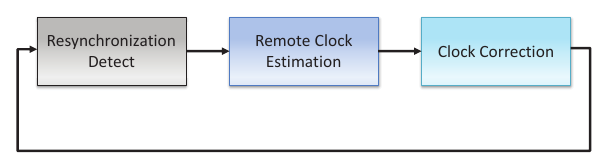
\includegraphics[width=0.8\textwidth]{img/TTA_resincronizacion_building_blocks.png}
%     \caption{Tres bloques que comprenden un algoritmo de resincronización. La imagen se extrajo de \cite{de2013overview}.}
%     \label{fig:TTA_resincronizacion_building_blocks}
% \end{figure}

% \begin{enumerate}
%     \item \textit{Resynchronization Detect}: Este bloque está dedicado a detectar e informar al nodo de que se va a ejecutar la resincronización.
%     \item \textit{Remote Clock Estimation}: Este es el bloque que realiza la cuenta del error entre el clock del nodo y la corrección a aplicar.
%     \item \textit{Clock Correction}: Este bloque corresponde a la aplicación de la corrección al clock local.
% \end{enumerate}

%Para la arquitectura de este trabajo, el primer bloque, \textit{Resynchronization Detect} simplemente consiste en ejecutar una tarea que estará incluida en el scheduling. El segundo bloque es el que realiza el cálculo y puede variar dependiendo de la implementación. Más adelante, se describirá el algoritmo utilizado. Por último, el bloque \textit{Clock Correction}, corresponde a aplicar la corrección al clock local. 
































% En la sección \ref{sec:sincronismo_TMR} se mencionó la necesidad del sincronismo entre los nodos y que esta se logra a partir de un intercambio de mensajes. Para la arquitectura propuesta, ese intercambio de mensajes se hace a través del mismo bus. Debido a que el medio es compartido, los nodos de la red deben tomar turnos para acceder al medio, de manera de que todos puedan enviar sus respectivos mensajes.

% Típicamente, una FCC ejecuta las mismas tareas relacionadas al control del vehículo, de manera periódica \cite{hiergeist2018implementation}:

% \begin{enumerate}
%     \item Lectura de los sensores.
%     \item Cálculo de la ley de control.
%     \item Aplicación del resultado a los actuadores.
% \end{enumerate}

% Debido a que se trata de un sistema de tiempo real, cada una de las FCCs debe realizar estas tareas en un período de tiempo dado. En la figura \ref{fig:task_scheduling_1} se muestra un gráfico con la secuencia de ejecución periódica de las tareas.

% \begin{figure}[H]
%     \centering
%     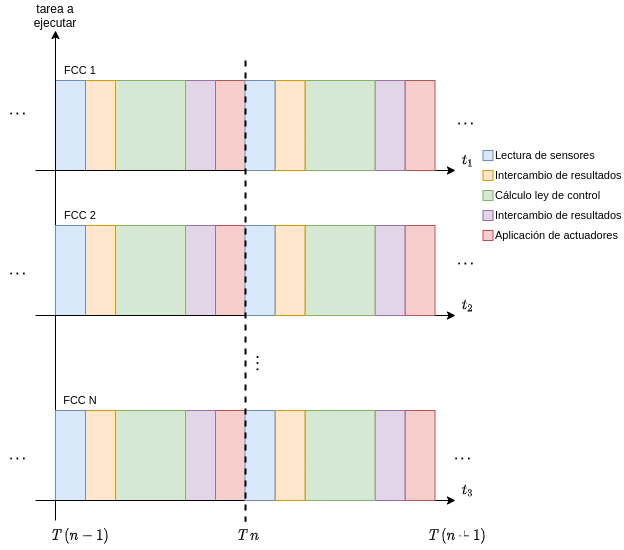
\includegraphics[width=0.7\textwidth]{img/task_scheduling_1.png}
%     \caption{El eje horizontal representa el paso del tiempo. Las barras de colores representan el tiempo dedicado a ejecutar cada tarea, como la lectura de sensores, cálculo de la ley de control, etc., de forma periódica. En la imagen se puede ver que las FCC 1, FCC 2, ..., FCC N se encuentran sincronizadas ya que realizan las tareas al mismo tiempo. }
%     \label{fig:task_scheduling_1}
% \end{figure}

% En un sistema con redundancias, como ya se mencionó, cada una de las FCCs realiza las mismas tareas. Además, estas intercambiarán resultados relacionados a mediciones de sensores y a valores de actuación para los motores con sus pares, justamente para enmascarar y tolerar las fallas. A partir de esto, se desprende que el intercambio de mensajes también corresponde a tareas que deben ejecutarse periódicamente y en un determinado período de tiempo acotado.

% Cada una de las computadoras de vuelo incluye un clock interno, el cual utiliza como base para cumplir con los tiempos de ejecución. Cuando se habla del sincronismo entre los nodos de la red, lo que se busca es que las ejecuciones de las N computadoras se encuentren coordinadas. Por ejemplo, en la figura \ref{fig:task_scheduling_2} se muestra un caso para dos computadoras de vuelo cuya ejecución se encuentra desfasada. Es fácil ver que este sistema nunca podrá cumplir con el objetivo de controlar el vuelo del UAV.

% \begin{figure}[H]
%     \centering
%     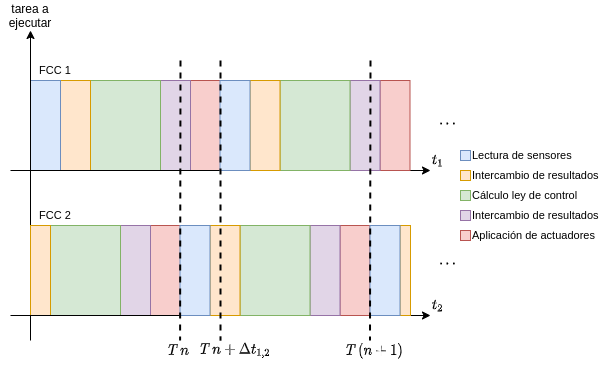
\includegraphics[width=0.7\textwidth]{img/task_scheduling_2.png}
%     \caption{Se muestra un ejemplo para dos FCCs. A diferencia de la figura \ref{fig:task_scheduling_1}, las FCC 1 y la FCC 2 se encuentran desincronizadas.}
%     \label{fig:task_scheduling_2}
% \end{figure}


% En la figura, se muestra que cuando la FCC 2 termina de enviar la señal de control a los actuadores (instante $T_n$), la FCC 1 se encuentra intercambiando resultados con la FCC 2. Debido a que la FCC 2 ya pasó dicha tarea, la FCC 1 no recibirá ningún valor de su par y asumirá erróneamente, que la FCC 2 se encuentra en un estado con alguna falla, ya que no responde. Si bien este ejemplo es muy simple, muestra la necesidad de la sincronización entre nodos de la red, siendo el motivo principal, el hecho de que el sistema es de tiempo real.

% %\subsection{Arquitectura Del Sistema: \textit{The Time-Triggered Architecture}}

% A partir de lo analizado hasta aquí, se enumeran los requerimientos más elementales del sistema:

% \begin{enumerate}
%     \item El sistema es de tiempo real, es decir, se requiere determinismo temporal en la ejecución de las tareas.
%     \item El sistema es redundante, por lo que cada nodo ejecuta las mismas tareas en paralelo y al mismo tiempo.
%     \item El uso del bus de comunicación obliga al uso de un protocolo de acceso al medio físico compartido (el bus) por turnos, que permita que todos los nodos tengan acceso a este.
% \end{enumerate}

% A continuación, se presentan distintas arquitecturas posibles para la implementación y se selecciona una de ellas, la \textit{Time-Triggered Architecture}\cite{kopetz2003time}, cuyas características se ajustan a los requerimientos.

% {\Large \textbf{{\color{red} ACÁ COMENTAR LAS ALTERNATIVAS DE LAS DISTINTAS ARQUITECTURAS, COMO SUPER LOOP, EVEN TRIGGERED CON RTOS, SIN RTOS Y TIME TRIGGERED. COMENTAR POR QUÉ ELIJO TIME TRIGGERED Y DESCARTO LAS DEMÁS. PONER CASOS DE TRABAJOS CON TTA. EN EL PAPER QUE USA TIME TRIGGERED BUSES HAY VARIOS EJEMPLOS }}}

% %\subsubsection{The Time-Triggered Architecture}

% En este tipo de arquitectura, el sistema en cuestión ejecuta sus tareas en instantes de tiempo predefinidos. Estas tareas pueden ser tales como tomar datos de un sensor, enviar un dato a otra parte del sistema o realizar algún cálculo. Este tipo de arquitectura es típicamente utilizada en aplicaciones de tiempo real críticas. {\textbf{{\color{red} PONER EJEMPLOS DE SISTEMAS CRÍTICOS CON TIME TRIGGERED ARCHITECTURE}}}. Esto es porque esta arquitectura vuelve al sistema predecible. Teniendo en cuenta lo mencionado en la sección \ref{subsec:introduccion_al_analisis_de_tolerancia_a_fallas}, que el comportamiento del sistema sea predecible lo vuelve más confiable y por ende más seguro.

% Existe otro criterio por el cual típicamente se prefiere este tipo de sistemas para aplicaciones de este estilo y tiene que ver con los procesos de validación que deben realizarse frente a entes reguladores. El hecho de tener un sistema cuyo comportamiento es altamente predecible, simplifica mucho su proceso de validación. \textbf{{\color{red} DESARROLLAR ESTA PARTE CON EJEMPLOS Y CITANDO DO-254, ETC}}.

% A continuación, se presenta brevemente los componentes y el funcionamiento de la arquitectura para el sistema de este trabajo. Pueden encontrarse trabajos\cite{kopetz2003time}\cite{kopetz1998time} y libros\cite{kopetz-2011} que explican formalmente esta arquitectura y sus distintos componentes con más detalle.

% Como ya se mencionó en las secciones anteriores, el sistema se compone de una serie de \textbf{nodos} interconectados a través de un \textbf{bus de comunicación}. Cada uno de los nodos ejecuta una serie de tareas con un \textbf{scheduling} predefinido por el paso del tiempo.

% \begin{figure}[H]
%     \centering
%     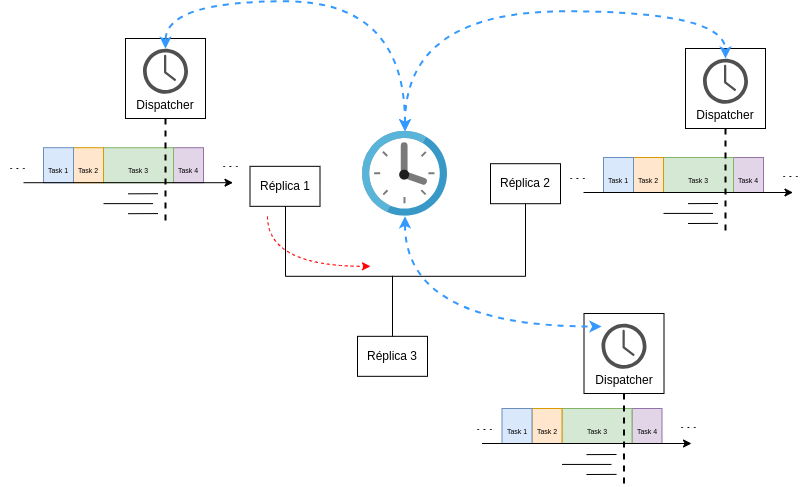
\includegraphics[width=\textwidth]{img/diagrama_TTA.png}
%     \caption{Se muestra un esquema que representa la arquitectura. Cada nodo tiene un \textit{clock} local, funcionando a partir de su propio cristal. Todos estos a su vez se sincronizan periódicamente con el \textit{global time}, representado por el reloj azul en el centro. En la imagen, el nodo 1 está enviando un mensaje por el bus. Los demás nodos saben previamente que deben esperar este mensaje.}
%     \label{fig:diagrama_TTA}
% \end{figure}

% Para que el comportamiento de los nodos sea consistente, estos deben estar \textbf{sincronizados}. Se define entonces una base de tiempo global a todos los nodos, denominada en la bibliografía \textbf{global time base}\cite[p.~51]{kopetz-2011}. Esta representa a un reloj que no existe físicamente, sino que es un acuerdo entre los nodos del sistema respecto a un reloj al que todos los nodos deben seguirle el ritmo. Para esto último, cada nodo tiene su propio \textbf{reloj local}.

% En la figura \ref{fig:diagrama_TTA} se muestra un esquema de la arquitectura \textit{Time Triggered}. Los tres nodos de la imagen, FCC1, FCC2 y FCC3 se encuentran sincronizados ejecutando la tarea \textit{Task 3}. Esta tarea implica que el nodo FCC1 envíe un mensaje por el bus, representado en la imagen por la flecha roja. En cuanto a los nodos FCC2 y FCC3, la \textit{Task 3} les dice que ellos deben escuchar el bus y esperar el mensaje proveniente del FCC1. Esto quiere decir que el comportamiento predefinido por el scheduler también define en qué instantes de tiempo cada nodo puede enviar un mensaje y en qué instantes de tiempo debe recibirlo. Con respecto a esto último, si en el ejemplo de la figura \ref{fig:diagrama_TTA} el nodo FCC1 presenta una falla y no envía el mesanje en el tiempo correspondiente, luego los nodos FCC2 y FCC3 no recibirán nada. Es común encontrar protocolos de comunicación donde este tipo de fallas se resuelven solicitando el reenvío del mensaje. Sin embargo, debido a que el sistema ya tiene un scheduling predefinido, esto no se permite ya que uno a priori no puede saber si habrá que hacer un pedido de reenvío de mensaje o no, lo que puede corromper el scheduling del sistema. Justamente, la \textit{Time-Triggered Architecture} busca que el sistema sea predecible.

% A continuación, se describe brevemente cada uno de los componentes de este tipo de sistema. Para una explicación más detallada, referirse a \cite{kopetz-2011} y \cite{kopetz2003time}.

% %\subsubsection{Bus de Comunicaciones}

% El bus de comunicaciones es el medio a través del cual los nodos intercambian información. Como se describió anteriormente, la arquitectura requiere la sincronización de los nodos para una ejecución consistente. Esto quiere decir que como mínimo, los nodos intercambian mensajes utilizados para la sincronización entre estos. Más allá de esto, en un sistema distribuido, lo más común es que haya un intercambio de información constante entre nodos.

% De manera de minimizar las colisiones y favorecer el cumplimiento en el timing del sistema de tiempo real, el envío y recepción de mensajes se implementa por turnos. Esto corresponde a un protocolo de acceso al medio denominado \textit{Time Division Multiple Access} (TDMA). En la figura \ref{fig:TDMA_esquema} se grafica esto para 3 nodos. Este protocolo define en qué instantes de tiempo cada uno de los nodos puede utilizar el medio físico y en cuáles no. Para que no haya colisiones, todos los nodos deben respetar ese timing, el cual se encuentra predefinido. 

% \begin{figure}[H]
%     \centering
%     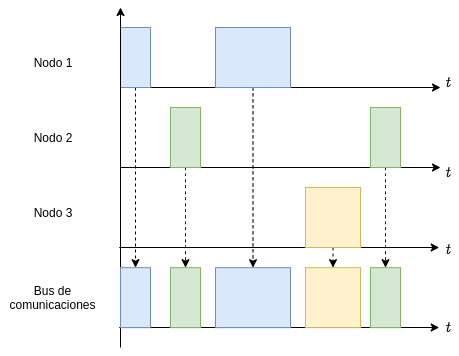
\includegraphics[width=0.7\textwidth]{img/TDMA_esquema.png}
%     \caption{El ejemplo muestra como los 3 nodos pueden compartir el bus de comuncaciones. Cada uno de ellos sabe en qué instante de tiempo enviar un mensaje y en qué instantes de tiempo no deben hacerlo y solamente pueden escuchar el bus. Para que esto funcione adecuadamente, los nodos deben estar sincronizados.}
%     \label{fig:TDMA_esquema}
% \end{figure}

% \textbf{{\color{red} ACÁ MENCIONAR ALGUNOS PROTOCOLOS COMO FLEXRAY O TTP/C QUE DE POR SÍ YA EJECUTAN UNA SINCRONIZACIÓN.}}

% En \cite{kopetz2003time} se define un elemento del nodo denominado \textit{Communication Network Interface}(CNI). Esta es una interfaz entre el software del nodo y el acceso al medio físico. Utilizando el protocolo de acceso al medio TDMA, el software del nodo \textit{pushea} un mensaje a la CNI. Es esta última la que se encarga de administrar los tiempos de envío y recepción. Es decir, mientras el nodo continua con sus tareas, la CNI se encarga de cumplir con el timing del envío del mensaje.

% \begin{figure}[H]
%     \centering
%     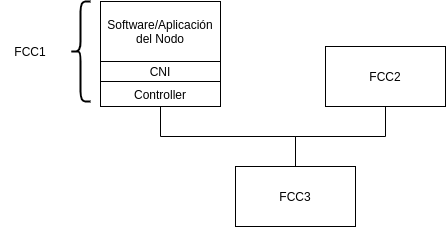
\includegraphics[width=0.6\textwidth]{img/TTA_Bus.png}
%     \caption{Misma imagen que \ref{fig:byzantine_bus_2}. Se muestra el detalle de los nodos, en el nodo FCC1.}
%     \label{fig:TTA_Bus}
% \end{figure}

% Al recibir un mensaje, ocurre algo similar. El software del nodo \textit{pollea} a la CNI en determinado instante de tiempo para obtener el mensaje recibido. Otra forma de implementar esto podría ser a través de una interrupción en el software, es decir, que cuando llege un mensaje nuevo, se dispare una interrupción en el software. El problema con esto es que se le quita determinismo al sistema.

% %\subsubsection{Nodos}

% Los nodos son la unidad elemental de los sistemas distribuidos, y también de la arquitectura \textit{Time-Triggered}. Estos son los que ejecutan las tareas y le dan vida al sistema. Los nodos se componen generalmente de un procesador (microcontrolador en el caso de este trabajo), un clock local (en este trabajo se implementa con un circuito oscilador con un cristal) una unidad de control de acceso al bus de comunicaciones y el software local al nodo. En la sección anterior además, se mencionó la existencia de un elemento llamado CNI, que comunica al software con el bus. Sumado a esto, el nodo a su vez contiene un scheduler, el cual se describie en la próxima sección.

% %\subsubsection{Scheduler}

% El sistema conformado por el conjunto de nodos y las comunicaciones entre ellos, se basa en un esquema de tareas que se encuentra predefinido. Esto se diferencia de sistemas de otras características como puede ser alguno con una interfaz con una persona. El caso más cercano puede ser el de un telófono celular, el cual tiene una pantalla que el usuario puede presionar en distintos lugares para abrir una aplicación, enviar un mensaje, etc. Cuando esto ocurre, el celular debe dar una respuesta casi inmediata. Este tipo de sistemas se llaman \textit{Event-Triggered} y son controlados por los eventos que pueden ocurrir. A priori, se asumen eventos asincrónicos, es decir, que pueden ocurrir en cualquier momento y en cualquier orden. A diferencia de esto, en un sistema \textit{Time-Triggered} los eventos no pueden ocurrir en cualquier momento. Mejor dicho, los eventos pueden ocurrir en cualquier momento, pero el sistema solamente prestará atención a esos eventos en un lapso de tiempo predefinido.

% En los sistemas operativos de tiempo real se definen una serie de tareas, las cuales utiliza un scheduler que determina cuál es la próxima tarea que corresponde ejecutar. Un sistema \textit{Time-Triggered} también define su comportamiento a través de tareas. La diferencia está en la estrategia utilizada por el scheduler. En el caso de un RTOS es común encontrar schedulers \textit{preemptive} con un sistema de prioridad. En un sistema \textit{Time-Triggered}, los schedulers pueden ser \textit{preemptive} o bien cooperativos. La ventaja de utilizar un scheduler cooperativo es nuevamente el determinismo en la ejecución de las tareas \cite[p.~247]{pont2008patterns}.

% %\subsubsection{Global Time y Sincronización}

% De forma de que el funcionamiento del sistema de tiempo real distribuido sea correcto, todos los nodos deben ejecutar sus tareas de forma consistente. Para ello, sus schedulers deben estar sincronizados. Para el caso de este trabajo, cada una de las FCCs debe encontrarse ejecutando la misma tarea al mismo tiempo. De esta forma pueden ejecutarse los algoritmos de votación para realizar tolerancia a fallas de hardware, como ya se describió anteriormente.

% Algunos sistemas distribuidos de tiempo real utilizan un clock maestro, implementado como un nodo de la red al que todos los demás nodos utilizan como referencia. Por ejemplo, la extensión del protocolo automotivo CAN, denominada Time-Triggered CAN (TTCAN) \cite{leen2002ttcan} utiliza esta estrategia. La desventaja de este método es que dicho clock maestro se convierte en un punto singular de falla: si este presenta una falla, habrá un error en la sincronización. 

% Otra forma es utilizar una \textit{global time base}\cite[p.~51]{kopetz-2011}. Esta se define como un acuerdo entre los nodos de la red respecto a una base de tiempo a utilizar como referencia. Como ya fue mencionado, cada nodo tiene un reloj interno propio, implementado con un cristal oscilador. Esta base de tiempos global puede implementarse por ejemplo utilizando un contador local. Cada nodo incrementa en uno el valor de esta variable, de forma periódica. Para que los nodos puedan utilizar esta variable como base de tiempos, todos los nodos deben tener el mismo número almacenado en su instancia local de dicha variable, al mismo tiempo.

% A priori, puede parecer que el hecho de que el valor del contador sea igual en cada nodo al mismo tiempo sea muy exigente. En la implementación, esto no es posible pero tampoco es necesario. Puede existir cierta precisión en la sincronización que dependiendo del hardware y del algoritmo de sincronización, se obtendrá un mejor o peor resultado.

% Luego de ejecutar el algoritmo de sincronización, los clocks de cada nodo quedarán sincronizados con cierta precisión $\Phi$. A medida que pase el tiempo, inevitablemente los clocks de cada nodo comenzarán a desfasarse uno del otro, lo cual incrementará el error. Por consiguiente, la sincronización debe ejecutarse de forma periódica. Esto se grafica en la figura \ref{fig:TTA_resincronizacion}.

% \begin{figure}[H]
%     \centering
%     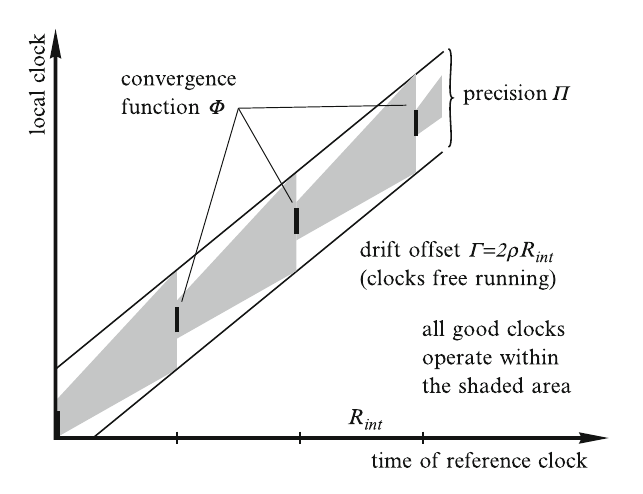
\includegraphics[width=0.7\textwidth]{img/TTA_resincronizacion.png}
%     \caption{El eje horizontal representa el paso del tiempo físico y el eje vertical el avance de cada clock local a cada nodo. El valor $R_{int}$ corresponde al período de resincronización. La imagen se extrajo de \cite[p.~67]{kopetz-2011}.}
%     \label{fig:TTA_resincronizacion}    
% \end{figure}

% Existen muchísimos algoritmos de resincronización. En \cite{anceaume1998performance} se puede encontrar un estudio que compara distintos tipos de algoritmos. Un planteo interesante de este trabajo es que los algoritmos de resincronización pueden dividirse en tres bloques básicos, figura \ref{fig:TTA_resincronizacion_building_blocks}, donde lo que varía es la implementación de cada bloque.

% \begin{figure}[H]
%     \centering
%     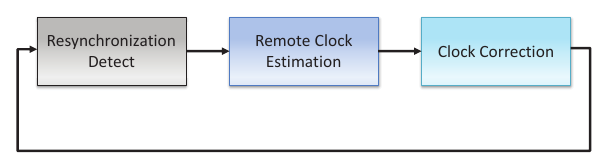
\includegraphics[width=0.8\textwidth]{img/TTA_resincronizacion_building_blocks.png}
%     \caption{Tres bloques que comprenden un algoritmo de resincronización. La imagen se extrajo de \cite{de2013overview}.}
%     \label{fig:TTA_resincronizacion_building_blocks}
% \end{figure}

% \begin{enumerate}
%     \item \textit{Resynchronization Detect}: Este bloque está dedicado a detectar e informar al nodo de que se va a ejecutar la resincronización.
%     \item \textit{Remote Clock Estimation}: Este es el bloque que realiza la cuenta del error entre el clock del nodo y la corrección a aplicar.
%     \item \textit{Clock Correction}: Este bloque corresponde a la aplicación de la corrección al clock local.
% \end{enumerate}

% Para la arquitectura de este trabajo, el primer bloque, \textit{Resynchronization Detect} simplemente consiste en ejecutar una tarea que estará incluida en el scheduling. El segundo bloque es el que realiza el cálculo y puede variar dependiendo de la implementación. Más adelante, se describirá el algoritmo utilizado. Por último, el bloque \textit{Clock Correction}, corresponde a aplicar la corrección al clock local. En general existen dos formas de realizar esto. La primera es pisando el contador existente con el nuevo valor calculado. Este método puede generar inconsistencias en la ejecución de las tareas del nodo \cite[p.~72]{kopetz-2011}. La forma que se prefiere es ir aplicando correcciones sucesivas conforme se van reajustando los clocks. Esto es algo similar a un algoritmo de control, donde se calcula un error y en función de dicho error, se aplica una corrección a la acción de control. En este último caso, la corrección puede implementarse por ejemplo dejando pasar más o menos tiempo para incrementar el contador del clock local.

\subsection{Implementación en Firmware}

%El objetivo de esta sección es explicar cómo se implementaron las características del sistema Time-Triggered Architecture. Por ejemplo, cómo se implementó el scheduler, la sincronización y la comunicación entre nodos.

%A continuación, se explica cómo se realizó la implementación de las características de la arquitectura mencionada en la sección anterior.

Para realizar pruebas con las computadoras de vuelo, se hizo una implementación en firmware de la arquitectura con las características mencionadas. Se utilizó el lenguaje de programación \textit{C}, junto con algunas bibliotecas de terceros desarrolladas en \textit{C++}, por ejemplo para uso del sensor IMU. 

%El diagrama de flujos de la figura  describe el funcionamiento.

Se comienza con una inicialización de los periféricos y sensores conectados, para luego pasar a un estado en el que se espera una orden para comenzar la ejecución del \textit{scheduler}. Esto puede ser a través de un comando externo enviado por el piloto remoto, algún mensaje por el bus CAN, o cualquier otro mecanismo.
%{\Large \textbf{{\color{red} IMAGEN DEL DIAGRAMA DE FLUJOS. ACLARAR A PATIR DE DÓNDE SE VUELVE TIME-TRIGGERED. SINO PUEDE SER UN DIAGRAMA MÁS GENÉRICO, CON UN RELOJITO Y UNA LISTA DE TAREAS.}}}
Es importante destacar que esto ocurre previo a la ejecución del scheduler, por lo que el sistema no tiene un comportamiento controlado por el tiempo. Previo a su ejecución, este se comporta como un sistema del tipo \textit{event-triggered}. Si bien se mencionó que esto tiene algunas características que perjudican la seguridad, el estado previo a la ejecución del \textit{scheduler} corresponde a una inicialización, por lo que no se compormete la seguridad del vehículo. En este estado, el UAV todavía se encuentra en tierra con sus motores apagados esperando una orden para comenzar su misión.

\subsubsection{Scheduler}

%Implementación de la clase del scheduler, implementación de la clase de las tareas, con herencia y creación de tareas particulares. Mención de herencia en C en el estándar ISO bla bla bla.

Para la implementación del \textit{scheduler} se tomó como referencia lo que se propone en \cite{pont2008patterns}. El autor utiliza una lista de tareas, un timer y una dispatcher que determina cuál es la siguiente tarea a ejecutar. Inicialmente la lista se encuentra vacía y deben agregarse las tareas pertinentes a la aplicación a ser desarrollada. El scheduler requiere que se reserve un periférico timer configurado para generar una interrupción por overflow. Cada vez que esto ocurre, se llama al dispatcher, el cual selecciona y ejecuta la próxima tarea.

Con el objetivo de darle mayor visibilidad al código, es decir que pueda entenderse el flujo de ejecución fácilmente, tanto el scheduler como las tareas se implementaron a partir de estructuras que emulan el comportamiento de una clase del lenguaje de programación \textit{C++}. Además, esto permite la reutilización de código, lo cual se aprovecha sobre todo para la creación de cada una de las tareas. En la figura \ref{fig:class_diagram} se muestra un diagrama de clases que relaciona al scheduler con las tareas a ejecutar. %Esto es otro aspecto que refuerza el objetivo de obtener un sistema cuyo comportamiento sea predecible y por ende seguro.

%Como ya fue mencionado en varias oportunidades, el hecho de que el comportamiento del sistema sea predecible lo vuelve más seguro. 

%Si el código puede leerse fácilmente, entonces puede entenderse el flujo de ejecución fácilmente, entonces es predecible y por ende seguro.

\begin{figure}[H]
    \centering
    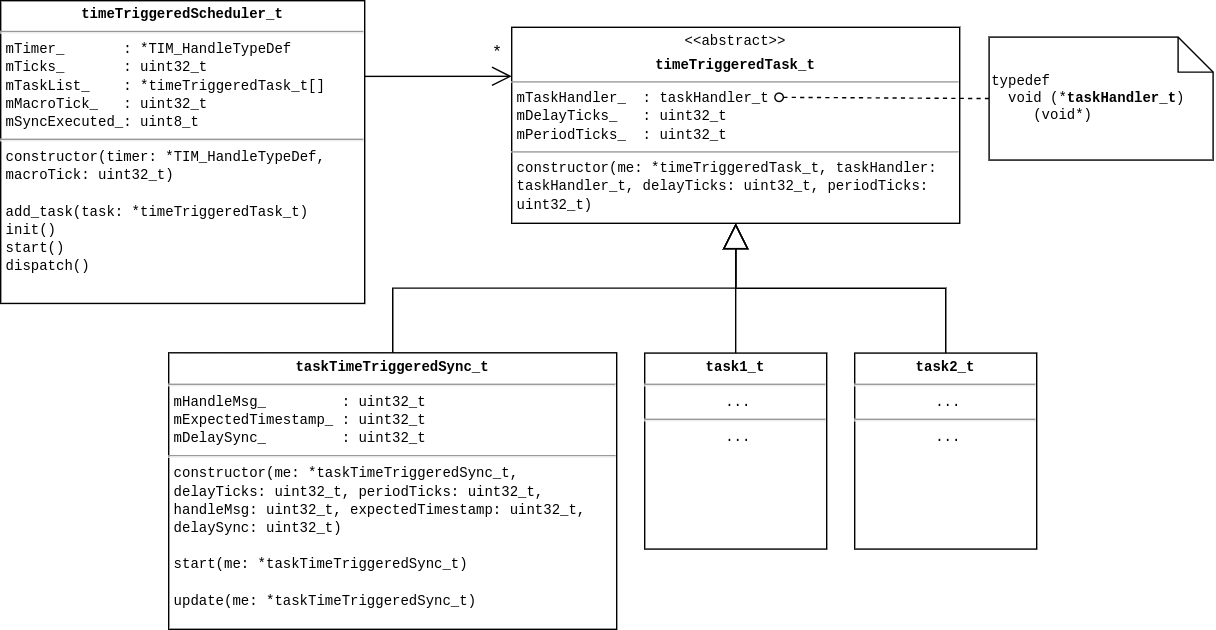
\includegraphics[width=\textwidth]{img/class_diagram.png}
    \caption{Diagrama de clases. La lista de tareas del scheduler se implementa como un arreglo de punteros. Cada una de las tareas del scheduler se crea a partir de una tarea base, \textit{timeTriggeredTask\_t}. Se muestra a modo de ejemplo la tarea encargada de ejecutar la resincronización.}
    \label{fig:class_diagram}
\end{figure}

%{\Large \textbf{{\color{red} IMAGEN DEL DIAGRAMA DE CLASE. MOSTRAR EL SCHEDULER, LA CLASE TIME TRIGGERED TASK Y LA RELACIÓN DE HERENCIA CON CADA TAREA.}}}

La clase \textit{timeTriggeredTask\_t} contiene una serie de atributos básicos que son aprovechados por el scheduler para determinar sus características temporales, en particular los atributos delay (\textit{mDelayTicks\_}) y período (\textit{mPeriodTicks\_}). Debido a que cada tarea tendrá sus propias características particulares, todas ellas se implementan a partir del uso de herencia. Si bien este aspecto es una característica que se asocia más con el lenguaje \textit{C++}, es posible emularlo en el lenguaje \textit{C} \cite[p.~32]{samek2008practical}.

El tiempo de ejecución se divide en intervalos discretos de duración fija, denominados ticks y en cada uno de ellos se llama al dispatcher. En la figura  se muestra un ejemplo de cómo el scheduler realiza la selección de la tarea a ejecutar. Como se mostró anteriormente, cada tarea cuenta con un atributo que indica su delay y su período. Estos atributos se miden en cantidad de ticks y son observos por el scheduler al momento de seleccionar la siguiente tarea a ejecutar.

{\Large \textbf{{\color{red} IMAGEN DE UN EJEMPLO DE SCHEDULER, DONDE SE VEA COMO SE VA DECREMENTANDO EL VALOR DEL ATRIBUTO DELAY Y QUE CUANDO LLEGA A 0 SE EJECUTA. luEGO SE LO VULEV EA CARGAR CON EL PERÍODO PARA LA PRÓXIMA EJECUCIÓN}}}

En cada llamado al dispatcher, se decrementa en 1 el atributo delay de cada tarea de la lista de tareas. Cuando se detecta que una tarea tiene un delay igual a 0, se selecciona la tarea y se la ejecuta. Al finalizar la ejecución, se carga el valor del período de dicha tarea en su atributo delay. De esta forma, queda definido el próximo instante de tiempo en el que será ejecutada nuevamente.

Una aclaración imporante es que la única interrupción que se ejecuta en todo el firmware es la del timer del scheduler. Ninguna de las tareas podrá hacer uso de las interrupciones de los distintos periféricos. Esto es porque, como fue mencionado anteriormente, todas las acciones deben tener un instante de ejecución predefinido con motivo de darle mayor determinismo al sistema.

\subsubsection{Comunicación a Través del Bus}

%Explicación de CNI, configuración del periférico CAN, identificación del nodo en el campo ID de la trama, configuración de filtros de hardware, funciones de transmisión y recepción. Tareas genéricas del scheduler que reciben o envían mensajes.

Dado que el comportamiento del sistema se encuentra predefinido, luego los mensajes, su información y sus correspondientes instantes de tiempo en los que se recibirán y en los que se enviarán, también. Para la implementación, se utiliza una lista estática de mensajes definida en tiempo de compilación. Cada entrada de la lista contiene información asociada a un mensaje distinto. Para esto se creó un tipo de dato \textit{CANmsg\_t} con los atributos que se muestran en la figura .

{\Large \textbf{{\color{red} IMAGEN CON LOS CAMPOS DE LA ESTRUCTURA CANMSG\_T.}}}

Como se puede ver, la lista de mensajes no almacena ningún aspecto relacionado a la temporalidad del mensaje. Para ello, la interfaz de comunicación implementada contiene dos métodos, uno para enviar y otro para recibir un mensaje, los cuáles deberán ser llamados en las distintas tareas que se agreguen al scheduler. En la figura  se muestra la interacción entre el bus de comunicaciones y el resto del sistema.

% En \cite{kopetz2003time} se define un elemento del nodo denominado \textit{Communication Network Interface}(CNI). Esta es una interfaz entre el software del nodo y el acceso al medio físico. Utilizando el protocolo de acceso al medio TDMA, el software del nodo \textit{pushea} un mensaje a la CNI. Es esta última la que se encarga de administrar los tiempos de envío y recepción. Es decir, mientras el nodo continua con sus tareas, la CNI se encarga de cumplir con el timing del envío del mensaje.

\begin{figure}[H]
    \centering
    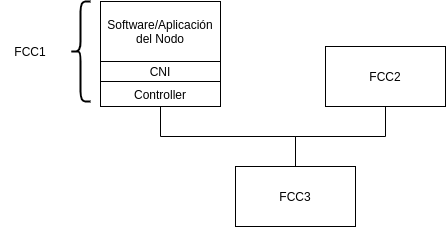
\includegraphics[width=0.6\textwidth]{img/TTA_Bus.png}
    \caption{Misma imagen que \ref{fig:byzantine_bus_2}. Se muestra el detalle de los nodos, en el nodo FCC1 {\color{red} ESTA IMAGEN SERÁ PARECIDA PERO HAY QUE HACERLA MÁS EXPLÍCITA}.}
    \label{fig:TTA_Bus}
\end{figure}

En los resultados que se presentarán más adelante, uno de los tipos de mensaje que se intercambian es acerca de la orientación del vehículo, estimada por cada réplica. Para lograr esto se define una tarea que ejecuta este cálculo y almacena el resultado en la tabla estática antes mencionada. Luego, cuando sea el momento de enviar este dato por el bus CAN, otra tarea consulta la tabla, obtiene la información y envía el mensaje a las demás réplicas. 

Cuando se recibe un mensaje, el firmware obtiene la información de este consultando al periférico durante la ejeución de la tarea correspondiente y almacenando el dato en la tabla interna. Más adelante, este dato podrá ser utilizado por otra tarea leyéndolo de la misma.

% configuración del periférico CAN, identificación del nodo en el campo ID de la trama, configuración de filtros de hardware

Para llevar adelante la comunicación a través del bus CAN, se utilizó el periférico del microcontrolador. Su funcionamiento puede describirse a partir de la figura  . Este se configuró para trabajar en su velocidad más alta, 1 MBit/s. La transmisión de mensajes se administra a través de 3 espacios de memoria presentes en el periférico, llamados mailboxes. Allí, el programa principal puede depositar mensajes de CAN, para que luego el periférico se encargue de transmitirlos por el bus. En caso de que la información que se quiera transmitir supere el tamaño máximo de un mensaje CAN, 8 bytes, este deberá partirse en varios mensajes. Para asegurarse de que estos se envíen en el orden correcto, el periférico permite que las mailboxes trabajen como una FIFO, asegurando el orden de los datos enviados.

{\Large \textbf{{\color{red} ESQUEMA DEL PERIFÉRICO CAN.}}}

Otro aspecto importante es que en caso de no poder inyectar el mensaje en el bus de comunicaciones, en su configuración por defecto el periférico no descartará el mensaje. Este será retenido hasta que pueda ser enviado. Este comportamiento perjudica gravemente el determinismo de las comunicaciones y no puede tolerarse. Es por esto que se deshabilitaron las retransmisiones automáticas y en caso de que la transmisión falle, se descartará el mensaje y se dará aviso al programa principal.

En cuanto a la recepción de mensajes, el funcionamiento es similar. En este caso además existe un mecanismo de filtroado de mensajes indeseados. Como fue mencionado en la sección \ref{sec:interfaz_CAN}, el campo identifier indica el contenido del mensaje CAN. La configuración de filtros permite que solamente se acepten mensajes con determinado valor en su campo identifier. Cada vez que se recibe un mensaje, este queda almacenado en otras mailboxes, las cuáles también se configuran para trabajar como FIFO.

% el periférico tiene una funcionalidad para uso de time-triggered communication, pero en una errata dice que no.

Una aclaración importante es que en la hoja de datos del microcontrolador utilizado, se menciona que este contiene el hardware necesario para utilizar el bus CAN con un funcionamiento \textit{time-triggered} \cite[p.~1295]{RM0385}. Sin embargo, el fabricante ST ofrece una errata \cite{STM32F746_errata} donde se aclara que esto no es así. Es por esto que tuvo que utilizarse el timer del scheduler para darle determinismo a la transmisión y recepción de mensajes.

\subsubsection{Sincronización}

% Como fue mencionado anteriormente, no se recomienda el uso de un sistema con un clock maestro, debido a que esto convierte a una de las réplicas en un punto singular de falla de todo el sistema. Lo correcto sería implementar un mecanismo donde se llegue a un consenso de la base de tiempos, entre cada réplica. Con motivo de simplificar las pruebas realizadas, en las pruebas realizadas en este trabajo se optó por utilizar una sincronización con un clock mestro. La implementación de un algoritmo distribuido forma parte del trabajo futuro a desarrollar. Lo implementado en este trabajo es suficiente para demostrar que la arquitectura que se propone puede implementarse con el hardware desarrollado.

Como fue mencionado anteriormente, algunos sistemas \textit{time-triggered} utilizan un clock maestro a partir del cual el resto de los miembros del bus toman como referencia para sincronizarse. Por ejemplo, esto corresponde al método de sincronización del protocolo TTCAN. Esto trae como desventaja el hecho de que el clock maestro se convierte en un punto singular de fallas de todo el sistema. 

En este trabajo, con el motivo motivo de simplificar las pruebas realizadas, se utiliza una sincronización con un clock maestro. Dentro del trabajo futuro a realizar, resta implementar un algoritmo distribuido. En este trabajo, es suficiente para demostrar que la arquitectura que se propone puede implementarse con el hardware desarrollado.

% Mencionar que la sincronización se ejecuta como una tarea periódica que se carga en el scheduler como cualquier otra. Dependiendo de si se trata del maestro o el esclavo, la tarea ejecuta una acción distinta. Si es maestro, simplemente envía un mensaje con un determinado ID. Si es esclavo, la tarea lee el mensaje recibido y consulta el valor del timer del scheduler. Luego se compara el valor leído vs el valor esperado. De esta forma es posible saber si la réplica está adelantada o atrasada. Finalmente se corrige la duración del tick actual. Esto es posible gracias a una configuración de un registro del timer. La próxima vez que se ejecuta el scheduler, se vuelve a la duración estándar.

Al igual que el resto de las funcionalidades, la sincronización se ejecuta como una tarea más del scheduler. Dependiendo de si se trata del maestro o del esclavo, la tarea ejecuta una acción distinta. En la figura  se resume el proceso de sincronización entre las réplicas. En el caso del maestro, primero se deja pasar un breve período de tiempo $t_{sync}$ y luego simplemente se envía un mensaje con un determinado ID = 0x01.

% Descripción del método, con un gráfico temporal y la flechita que corrige la duración del tick.
{\Large \textbf{{\color{red} IMÁGENES CON EL PROCESO DE SINCRONIZACIÓN Y CORRECCIÓN. ACLARAR LOS NOMBRES DE TODAS LAS DURACIONES DE TODOS LOS PERÍODOS DE TIEMPO, PARA QUE SEA BIEN CLARO.}}}

En cuanto a las demás réplicas, cuando estas ejecuten su tarea de sincronización, estarán esperando a recibir el mensaje proveniente del maestro. En ese momento, consultarán el valor del contador del timer utilizado para el scheduler y obtendrán un valor $t_{timestamp}$. A partir de la comparación de este valor contra el valor esperado $t_{sync}$, se obtendrá un error de sincronización, el cual deberán utilizar para corregir sus propios schedulers.

%Finalmente se corrige la duración del tick actual. Esto es posible gracias a una configuración de un registro del timer. La próxima vez que se ejecuta el scheduler, se vuelve a la duración estándar.

Como se muestra en la figura , el paso de corrección se aplica alargando o achicando la duración del tick actual. El periférico del timer utilizado en el microcontrolador de este trabajo permite modificar el valor del registro de overflow, TIMx\_ARR, mientras este se encuentra corriendo. Esto se realiza a partir de setear el bit ARPE = 0 (auto-reload preload bit) en el registro TIMx\_CR1 \cite[p.~745]{RM0385}. El valor a setear en el registro TIMx\_ARR debe ser $t_{tick} + \Delta t_{sync}$, donde $t_{tick}$ es la duración de un tick durante el funcionamiento normal y $\Delta t_{sync} = t_{timestamp} - t_{sync}$.
Finalmente para retomar el normal funcionamiento, cada réplica debe volver a corregir el valor del registro TIMx\_ARR con el valor nominal de $t_{tick}$. De esto último se encarga el scheduler, en el momento en que se llama al dispatcher en el siguiente tick luego de haber ejecutado la tarea de sincronización.

\subsubsection{Tarea de Ejemplo: Adquisición de Datos del Sensor IMU}\label{sec:tarea_de_ejemplo_adquisicion_datos_IMU}

% El objetivo de esta sección es dar una primera muestra de que lo que se implementó funciona como se dijo que debe funcionar. Para eso, quiero poner capturas de analizador lógico, mostrando que los mensajes se envían en los tiempos configurados y que el intervalo de tiempo entre mensajes se mantiene estable gracias al efecto de la sincronización periódica.

% La aplicación tiene que ser que se obtienen datos de la IMU y se envían por CAN. Hay que poner una imagen que muestre el timing de las tareas (para esto usar una imagen como la que hice con el script de python). Explicar que la tarea obtiene los datos del sensor, los formatea y los guarda en la tabla. Luego, otra tarea lo envía y en el receptor otra lo recibe y lo almacena internamente.

En esta sección se muestra un ejemplo utilizando las 3 réplicas de la computadora de vuelo, donde cada una de ellas obtiene datos de su correspondiente sensor IMU, de manera sincronizada. Luego, estas envían sus respectivas mediciones a través del bus de comunicaciones. Utilizando un analizador lógico se toman mediciones de los tiempos en el bus y se muestra el efecto de la sincronización.

% Hay que mostrar el funcionamiento sin sincronización, para que se vea que se rompe todo. Para esto, hay que usar una captura de analizador lógico, sí o sí. Acá hacer énfasis en que las placas se van desincronizando periódicamente. Incluso puedo poner un gráfico que releve todos los instantes de tiempo medidos con el analizador lógico. 

Las tareas a ser ejecutadas por el scheduler se muestran en la tabla \ref{tab:schedule_adquisicion_IMU} junto con sus características temporales. La tarea ``Obtener dato IMU'' es la encargada de obtener el dato del sensor, darle formato y almacenarlo en la tabla interna de mensajes de cada réplica. Por otro lado, la tarea ``Enviar dato IMU'' consultará dicha tabla y enviará el mensaje por el bus CAN. Además, se incorporan otras 2 tareas auxiliares. La tarea ``Heartbeat'' simplemente se encarga de parpadear un LED cada 1 segundo, dando una indicación de que el scheduler está funcionando adecuadamente.

\begin{table}[H]
    \centering
    \begin{tabular}{|l|c|c|}
        \hline
        \multicolumn{3}{|c|}{Duración Tick = 1 ms}\\
        \hline
        Tarea & Período [ticks] & Delay [ticks]\\
        \hline
        Heartbeat        & 1000 & 0 \\
        Watchdog         & 1    & 0 \\ 
        Obtener dato IMU & 100  & 1 \\
        Enviar dato IMU  & 100  & 2 \\
        \hline
    \end{tabular}
    \caption{Set de tareas para la adquisición y envío de datos de la IMU para la réplica 1.}
    \label{tab:schedule_adquisicion_IMU}
\end{table}

Para detectar cuándo una réplica no cumple con el timing de su set de tareas, se utiliza el periférico independent watchdog (IWDG) del microcontrolador. El timeout configurado es de $1.5 \ ms$. La tarea ``Watchdog'' se ejecuta cada $1 \ ms$ y es la encargada de evitar el reinicio del microcontrolador. En caso de que esto suceda, puede decectarse leyendo un registro del microcontrolador. En dicho caso, simplemente se encederá un LED y se entrará en un modo donde no se ejecutará ninguna acción, denominado fail-silent.

Las tareas de la tabla \ref{tab:schedule_adquisicion_IMU} pueden ubicarse temporalmente en un gráfico como el de la figura \ref{fig:grafico_hyperperiod_adquisicion_IMU}. Por una cuestión de claridad, solamente se muestran los primeros 10 ms de ejecución. 
 
\begin{figure}[H]
    \centering
    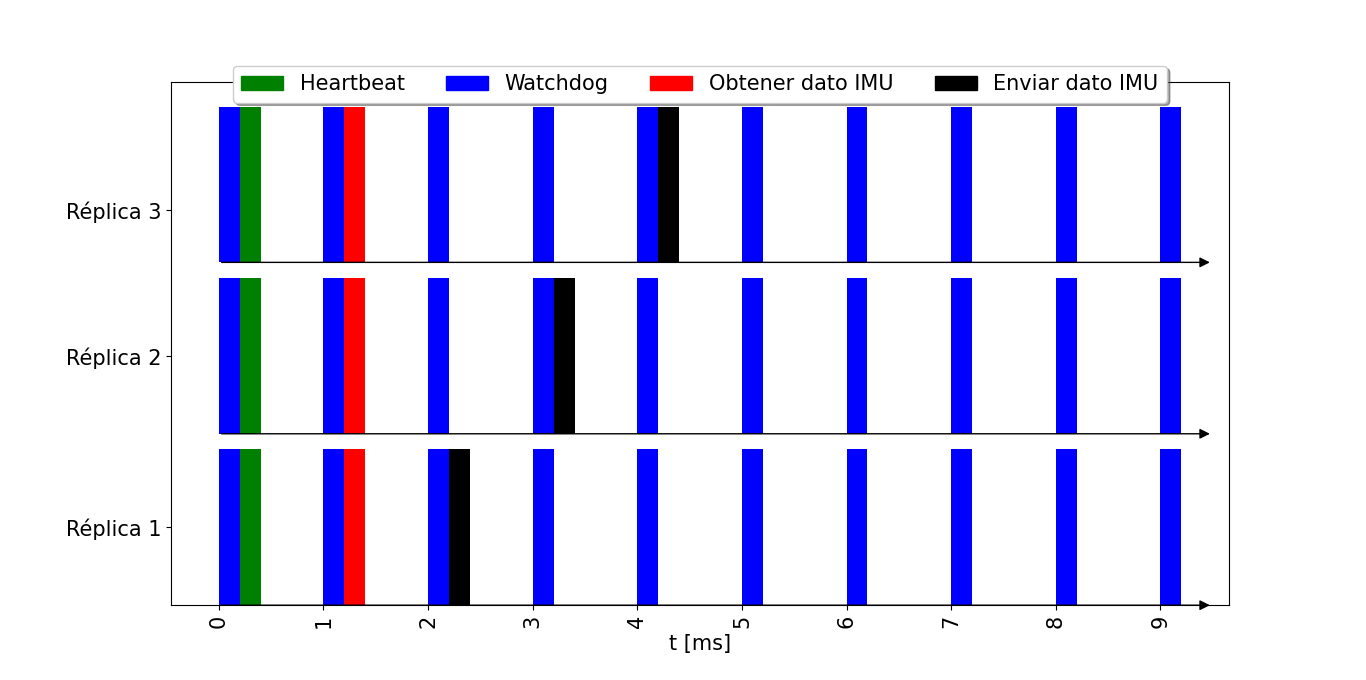
\includegraphics[width=\textwidth]{img/grafico_hyperperiod_adquisicion_IMU.png}
    \caption{Se muestran los primeros 10 ms de ejecución del scheduler. Existe una diferencia entre las 3 réplicas de 1 tick de separación en la tarea de envío de datos por el bus CAN. En cuanto a la tarea ``Watchdog'', esta se ejecuta en cada tick, evitando que se reinicie el microcontrolador.}
    \label{fig:grafico_hyperperiod_adquisicion_IMU}
\end{figure}

{\Large \textbf{{\color{red} COMPLETAR UNA VEZ QUE LLEGUE EL NUEVO TESTER.}}}

% Captura de analizador lógico
% Captura de analizador lógico mostrando que se rompe el schedule
% Comentar que agregando la sincronización se arregla
% Captura de analizador lógico mostrando que esta vez el schedule no se rompe
% Gráfico hecho por mi, mostrando cómo cambia con sincronización vs sin sincronización.

\subsection{Pruebas Realizadas}

%Se describe el setting común de las pruebas: Que las 3 placas calculan pitch y roll, luego lo comparten, comparan y se obtienen los residuos. Las fallas se inyectan articialmente. En cada sección se explica la característica de la falla en particular.

%Una de las tareas que siempre estará presente es la del INS. En esta sección se muestra un ejemplo de uso de la arquitectura propuesta, donde se utiliza la IMU 

%Para realizar una prueba de las capacidades de tolerancia a fallas del sistema, se implementó un sistema de validación de datos para un sensor en particular, en este caso la IMU, la cual provee datos a la tasa más alta y aporta los datos escenciales para la estabilidad del vehículo. La arquitectura se basa en un principio típicamente usado: considerando que existen tres sensores del mismo tipo y características, se comparan los datos adquiridos de a pares, y aquel sensor que difiera con respecto a los otros dos se considera en falla. [13], [14].

Para demostrar las capacidades de tolerancia a fallas de todo el sistema, se presentan una serie de pruebas realizadas para la detección de fallas en el sensor IMU. Durante la ejecución del scheduler, las réplicas intercambian resultados de estimaciones de los ángulos de pitch y roll, obtenidas a partir de un filtro complementario \cite{Pose2014}. Estas comparan sus resultados con los de sus pares y luego aquella que difiera con respecto a las demás se considera en falla. Utilizando este método y a partir de la arquitectura propuesta, es posible detectar la falla de 1 de las réplicas de forma simultánea.

En la tabla \ref{tab:schedule_pruebas_realizadas} se muestran las tareas con sus características temporales y en la figura \ref{fig:grafico_hyperperiod_pruebas_realizadas} se muestra un gráfico temporal. A partir de esta secuencia, cada réplica obtiene una nueva estimación de ángulos de pitch y roll cada 100 ms.

\begin{table}[H]
    \centering
    \begin{tabular}{|l|c|c|}
        \hline
        \multicolumn{3}{|c|}{Duración Tick = 1 ms}\\
        \hline
        Tarea & Período [ticks] & Delay [ticks]\\
        \hline
        Heartbeat                 & 1000 & 0 \\
        Watchdog                  & 1    & 0 \\ 
        Obtener dato IMU          & 100  & 1 \\
        Filtro Complementario     & 100  & 2 \\
        Enviar pitch y roll       & 100  & 3 \\
        Recibir pitch y roll de 2 & 100  & 4 \\
        Recibir pitch y roll de 3 & 100  & 5 \\
        Calcular residuos         & 100  & 6 \\
        Enviar residuos           & 100  & 7 \\
        Recibir residuos de 2     & 100  & 8 \\
        Recibir residuos de 3     & 100  & 9 \\
        Sincronización            & 1000 & 450 \\
        \hline
    \end{tabular}
    \caption{Set de tareas correspondiente a la réplica 1, para las pruebas realizadas.}
    \label{tab:schedule_pruebas_realizadas}
\end{table}

\begin{figure}[H]
    \centering
    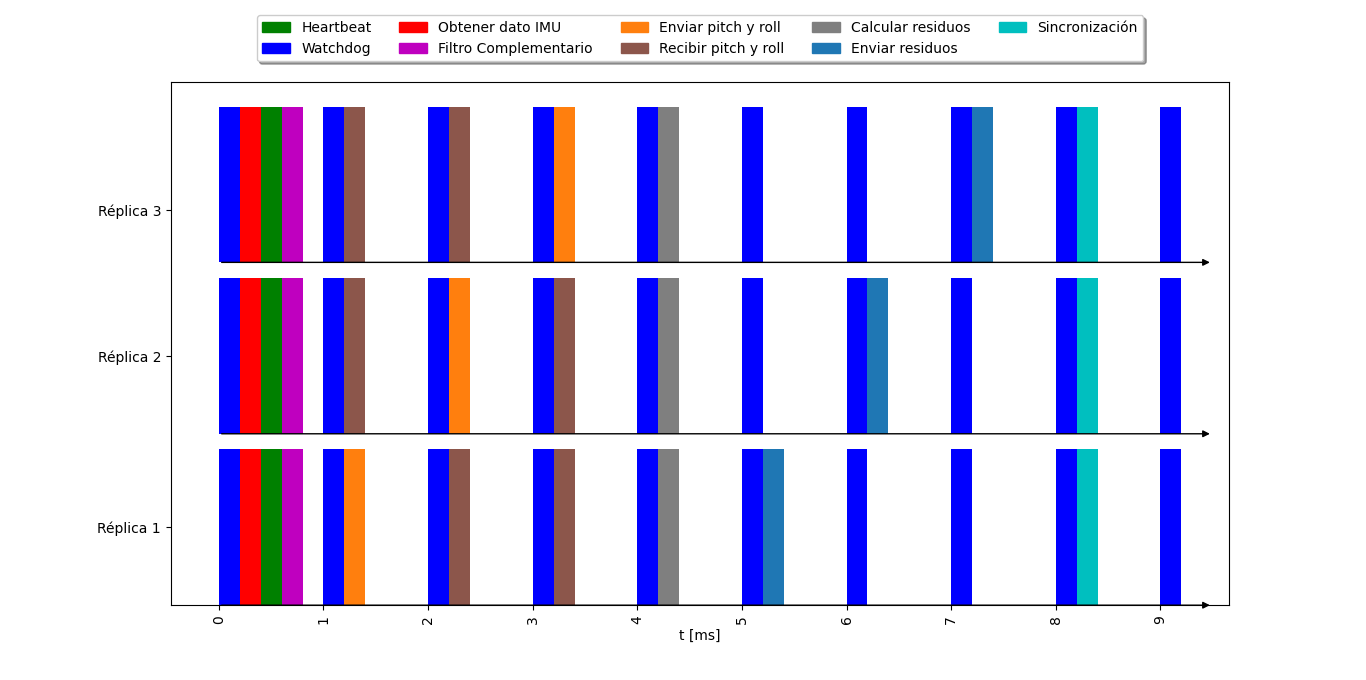
\includegraphics[width=\textwidth]{img/grafico_hyperperiod_pruebas_realizadas.png}
    \caption{Se muestran los primeros 12 ms de ejecución del scheduler. Por cuestiones de visualización no se muestra la tarea de sincronización, sin embargo esta se encuentra en el scheduler y se ejecuta cada 1 segundo, con un delay inicial de 450 ms.}
    \label{fig:grafico_hyperperiod_pruebas_realizadas}
\end{figure}

% Al igual que el ejemplo presentado en la sección \ref{sec:tarea_de_ejemplo_adquisicion_datos_IMU}, cada una de las réplicas tomará mediciones de su sensor de manera periódica.


% Breve mención al filtro complementario.
Mientras que la tarea ``Obtener dato IMU'' se encarga de consultar al sensor y obtener las mediciones de acelerómetros y giróscopos, la tarea ``Filtro Complementario'' realiza el procesamiento y obtiene una nueva estimación de los ángulos de pitch y roll. Este filtro realiza una estimación combinada, fusionando los datos de los acelerómetros y giróscopos. Se aplica un filtro pasa bajos a la estimación utilizando las mediciones de acelerómetro, debido a que sus mediciones son muy ruidosas. En cuanto a las mediciones de giróscopos, estas poseen un sesgo el cual se agrava por efecto de la integración. Es por esto que se aplica un filtro pasa altos a la estimación por giróscopos. Finalmente, se suman ambos resultados para obtener una mejor estimación, representados por las siguientes ecuaciones, donde $\theta[n]$ es el ángulo de pitch y $\phi[n]$ es el ángulo de roll:

\begin{subequations}
    \begin{align}
        \theta[n] &= \alpha \ atan_2(-a_x[n], \sqrt{a_y^2[n]+a_z^2[n]}) + (1 - \alpha) \left( \Delta T \ g_y[n] + \theta[n-1] \right)\\
        \phi[n] &= \alpha \ atan_2(a_y[n], a_z[n]) + (1 - \alpha) \left( \Delta T \ g_x[n] + \phi [n-1] \right)
    \end{align}
\end{subequations}

El valor $\alpha$ es un parámetro de ajuste del filtro, con un valor entre 0 y 1. Para las pruebas realizadas fue configurado con un valor de $0.025$.

% Explicacion de los residuos y cómo sirve para detectar la falla.
Seguido de esto, hay un período de intercambio de resultados de las estimaciones, a través del bus CAN. Esto corresponde a las tareas ``Enviar pitch y roll'' y ``Recibir pitch y roll'', las cuales permiten que todas las réplicas tengan una copia de las estimaciones de sus pares. Estos resultados se comparan en el tick 6, cuando se ejecuta la tarea ``Calcular residuos''. Se llama residuo a la diferencia entre cualquier par de resultados obtenido por las réplicas. Así, se obtienen 6 residuos, 3 para el ángulo de pitch y 3 para el ángulo de roll:

\begin{subequations}
    \begin{align}
        r_{1,2}^\theta[n] &= \left| \ \theta_1[n] - \theta_2[n] \ \right|\\
        r_{1,2}^\phi[n]   &= \left| \ \phi_1[n]   - \phi_2[n]   \ \right|\\
        r_{1,3}^\theta[n] &= \left| \ \theta_1[n] - \theta_3[n] \ \right|\\
        r_{1,3}^\phi[n]   &= \left| \ \phi_1[n]   - \phi_3[n]   \ \right|\\
        r_{2,3}^\theta[n] &= \left| \ \theta_2[n] - \theta_3[n] \ \right|\\
        r_{2,3}^\phi[n]   &= \left| \ \phi_2[n]   - \phi_3[n]   \ \right|
    \end{align}
\end{subequations}

En caso de que todas las réplicas obtengan resultados consistentes, los residuos tendrán valores cercanos a 0. Estos nunca alcanzarán un valor exactamente 0, debido a diferencias entre los sensores y a errores de cuantización. Por otro lado, si ocurre una falla en una de las IMUs, la estimación del pitch y/o roll de esa réplica divergirá con respecto a las demás. Esto generará que los valores de 2 de los residuos se alejen de cero, indicando cuál es el sensor en falla.

% Mencionar que los residuos se envían por el bus solo para ser loggeados con el analizador lógico para mostrarse acá.
Con motivo de observar el valor de los residuos, se agrega una tarea ``Enviar residuos'' donde cada réplica envía por el bus CAN los residuos que calcularon. Estos se loggean en una PC, utilizando un analizador lógico el cual registra todos los mensajes intercambiados en el bus CAN.

% Explicar cómo es que se implementa la inyección de falla, brevemente.
En los resultados que se presentan a continuación, todas las fallas fueron inyectadas de manera artificial, con el objetivo de emular un determinado comportamiento del sensor IMU. La inyección de la falla siempre se aplica en la misma tarea ``Obtener dato IMU'', antes de guardar las mediciones en la tabla de cada réplica.

%Para ello se configuraron los tres nodos de manera idéntica, para adquirir datos de acelerómetros y giróscopos de la IMU a una frecuencia de prueba de 10 Hz. Para evitar la desincronización entre placas, se toma como referencia el reloj del nodo 1, quien envía periódicamente cada 1 s un mensaje a los demás nodos para sincronizar sus relojes. Adquiridos los datos, en cada placa se ejecuta un filtro complementario para estimar los ángulos de roll y pitch, que son las rotaciones de la placa en el eje x que apunta hacia la nariz del vehículo, y en el eje y que apunta hacia la derecha, respectivamente. Luego, cada nodo publica mediante el bus CAN los datos de pitch y roll calculados, con lo cual todos los nodos adquieren la orientación calculada por los demás. Finalmente, cada nodo calcula los residuos entre las estimaciones del pitch de dos nodos como resi,j = |i - r | , i, j = 1, 2, 3, y los residuos de roll de manera análoga. Todos los residuos tendrán valores cercanos a cero en caso que los nodos obtengan mediciones consistentes. Si ocurre una falla en una de las IMUs, la estimación del pitch y/o roll de ese nodo divergirá con respecto a las demás, resultando en dos residuos cuyos valores se alejan de cero, lo cual permitirá conocer cuál es el sensor en falla. En las Figs. 5 y 6 se observa un experimento donde a los 10 s de iniciado, se inyecta un sesgo artificial de 10 ◦ s-1 en la medición del giróscopo en el eje x del nodo 2. Esto causa una estimación del ángulo de roll errónea en el nodo, que resulta en un sesgo constante respecto de los otros dos nodos, mientras que la estimación de pitch no se ve afectada. En el caso de los residuos, los de pitch no se ven afectados por la falla, mientras que los residuos que involucran al nodo 2 divergen rápidamente, permitiendo identificar el origen de la falla.

\subsubsection{Funcionamiento Sin Fallas}

% Mostrar cómo es la prueba con dibujitos, que dura 60 segundos, que se hace a mano y en qué posiciones se orienta durante cuánto tiempo (esto podría ir en la parte de funcionamiento sin fallas quizás)

En este primer caso no se inyectó ninguna falla en las mediciones de la IMU. Se ejecutó el set de tareas antes mencionado durante 60 segundos, orientando a las réplicas siguiendo el esquema de la figura \ref{fig:orientaciones_prueba}. Para que la orientación de las réplicas fuera la misma en todo momento, estas se apilaron con una serie de soportes, como se muestra en la figura \ref{fig:pruebas_stackeadas}.

\begin{figure}[H]
    \centering
    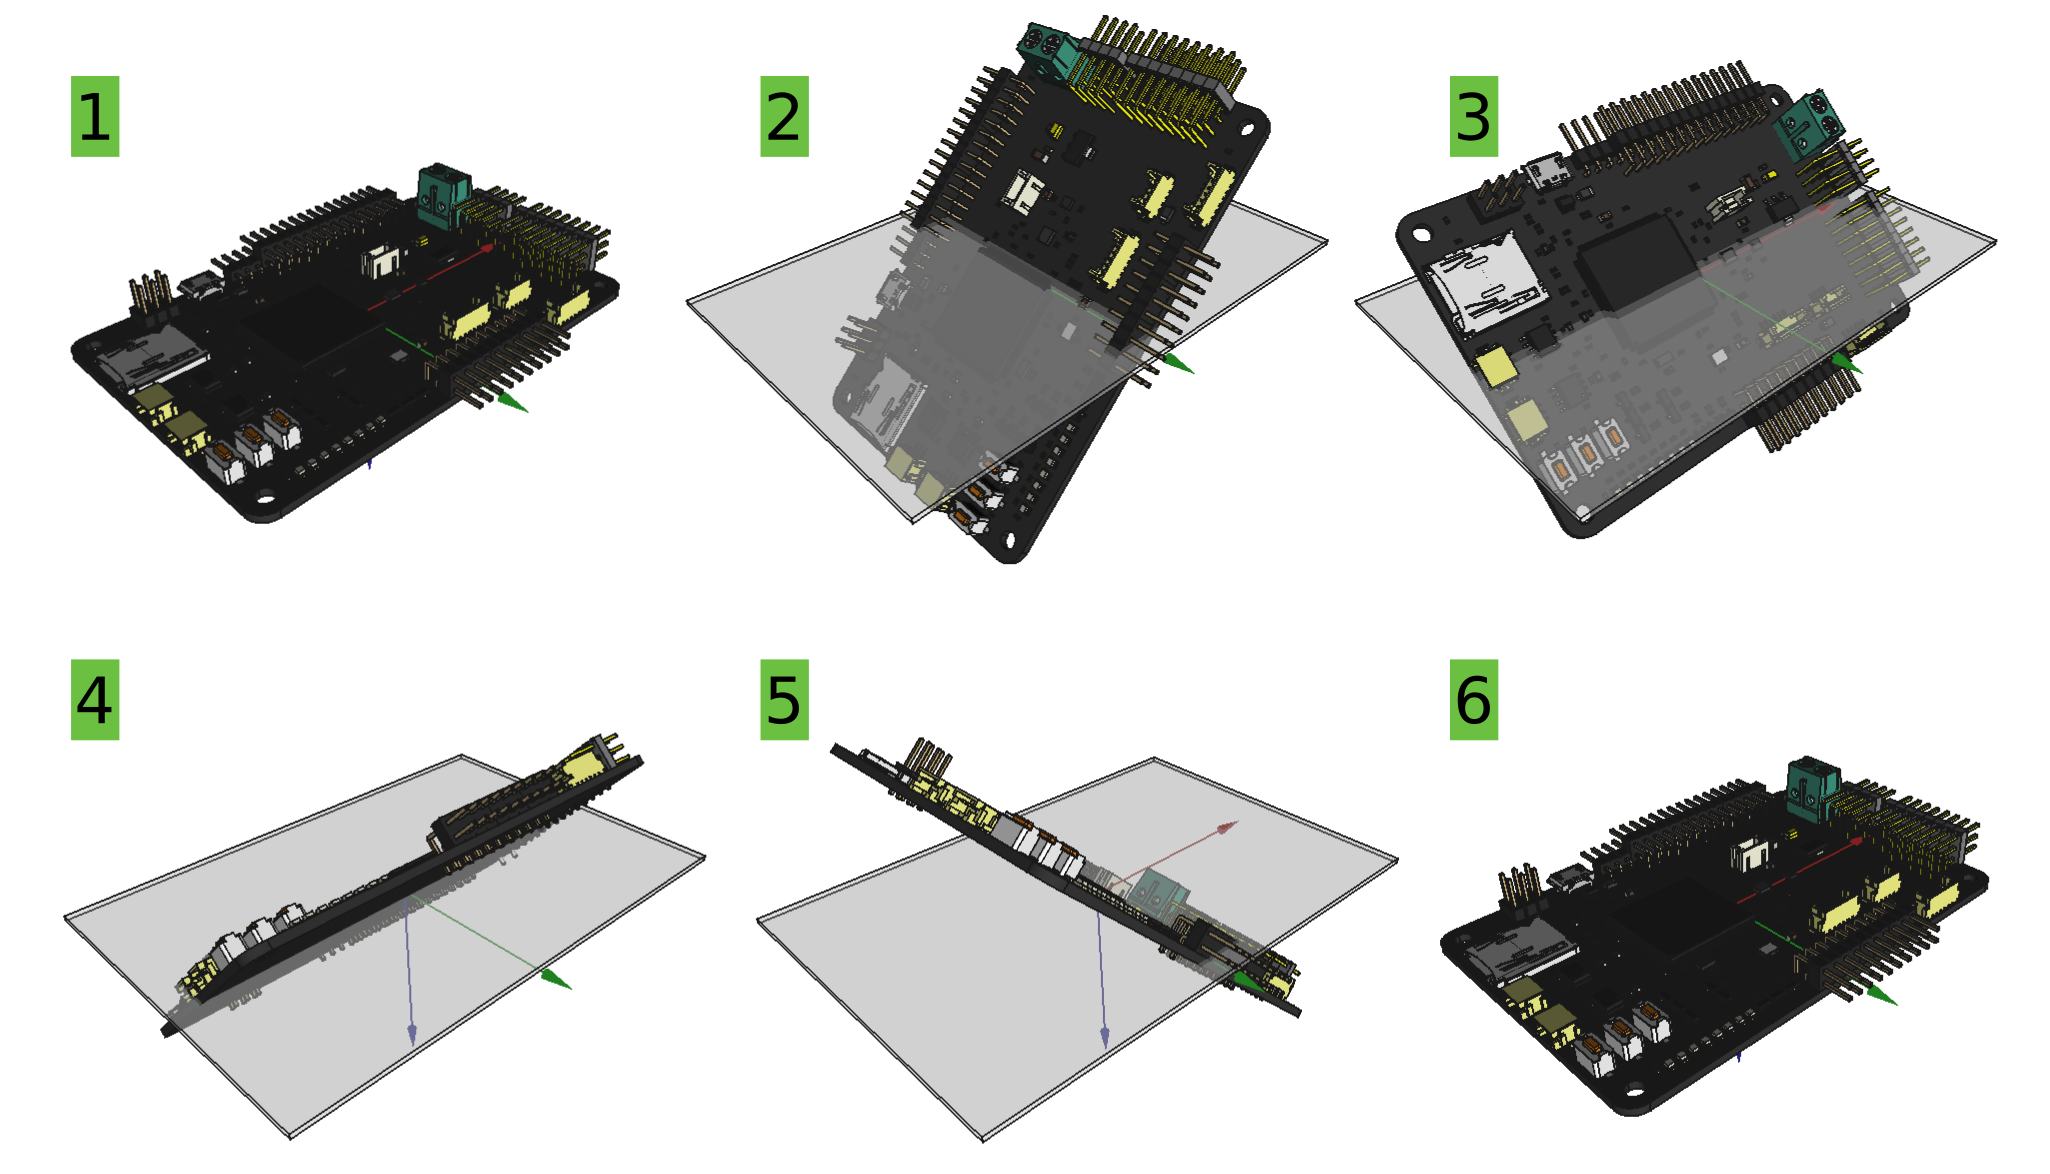
\includegraphics[width=0.8\textwidth]{img/orientaciones_prueba.png}
    \caption{Durante los primeros 10 segundos, las réplica se mantienen como en la orientación 1. Luego se continua con 2 durante otros 10 segundos, y así sucesivamente hasta finalizar en 6. Cada una de las orientaciones que se muestran corresponden a una rotación de aproximadamente 45$^o$.}
    \label{fig:orientaciones_prueba}
\end{figure}

\begin{figure}[H]
    \centering
    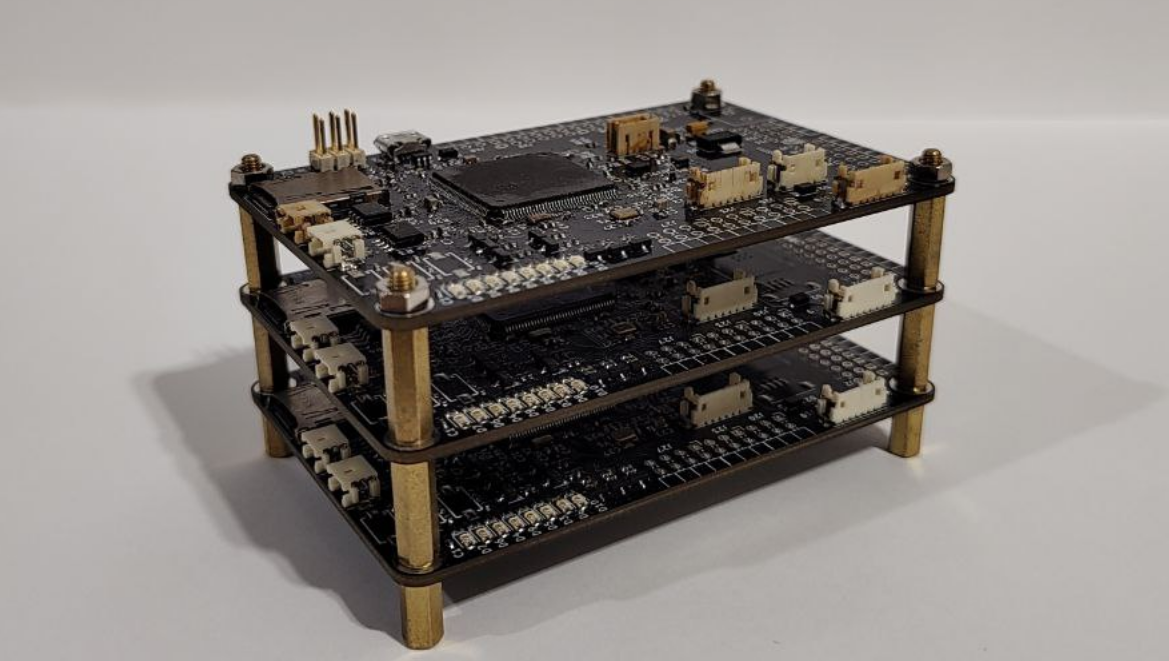
\includegraphics[width=0.7\textwidth]{img/pruebas_stackeadas.png}
    \caption{Se muestran las 3 réplicas apiladas.}
    \label{fig:pruebas_stackeadas}
\end{figure}

%{\Large \textbf{{\color{red} FOTO DE LAS PLACAS STACKEADAS EN LA BASE. TIENE QUE SER UNA FOTO PARA MOSTRAR ALGO VIVO, REAL.}}}

%{\Large \textbf{{\color{red} IMAGEN CON LAS POSICIONES DE LAS PLACAS. ESTA SÍ PUEDE SER UN 3D.}}}

{\Large \textbf{{\color{red} COMPLETAR UNA VEZ QUE LLEGUE EL NUEVO TESTER.}}}

% Acá también graficar resultados de sincronización

\subsubsection{Bias en Valores de Giróscopo}

{\Large \textbf{{\color{red} COMPLETAR UNA VEZ QUE LLEGUE EL NUEVO TESTER.}}}

\subsubsection{Saltos Aleatorios en Valores de Giróscopo}

{\Large \textbf{{\color{red} COMPLETAR UNA VEZ QUE LLEGUE EL NUEVO TESTER.}}}

\subsubsection{Medición Constante e Invariante de Acelerómetros y Giróscopos}

{\Large \textbf{{\color{red} COMPLETAR UNA VEZ QUE LLEGUE EL NUEVO TESTER.}}}

\subsubsection{Mediciones Inconsistentes de Acelerómetro}

{\Large \textbf{{\color{red} COMPLETAR UNA VEZ QUE LLEGUE EL NUEVO TESTER.}}}


%\subsection{Simplificación del Problema de Tolerancia a Fallas Arbitrarias de Hardware}

% En sistemas de tiempo real para aplicaciones \textit{safety-critical}, es común encontrar sistemas distribuidos con comunicación a través de un bus. Por ejemplo en los automóviles, los nodos que se encuentran repartidos por todo el vehículo se comunican a través de redes como CAN\cite{specification1991bosch} o FlexRay\cite{nxpAN12233}. Todos los nodos de la red se encuentran conectados al mismo bus de comunicación, por lo que cuando un nodo envía un mensaje a través del bus, todos los demás nodos reciben el mismo mensaje.

% \begin{figure}[H]
%     \centering
%     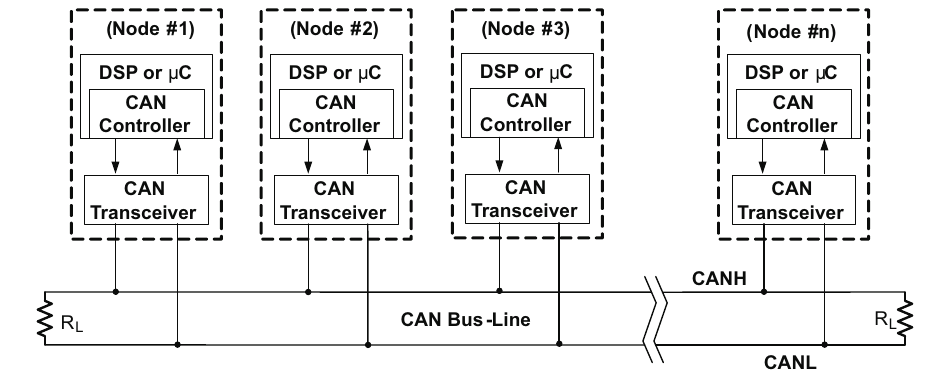
\includegraphics[width=\textwidth]{img/red_CAN.png}
%     \caption{Todos los nodos se encuentran conectados al mismo bus de comunicaciones. En el caso del bus CAN, se compone de dos cables, CAN-H y CAN-L, terminados en sus extremos por resistencias de adaptación. La imagen se extrajo de \cite{texasSLOA101B}.}
%     \label{fig:red_CAN}
% \end{figure}

% Esto presenta una diferencia respecto de lo planteado en \textit{The Byzantine Generals Problem}, ya que la existencia de un bus común a todos los nodos automáticamente elimina la posibilidad de que uno de los miembros de la red pueda enviar información diferente a sus pares. Puede compararse la figura \ref{fig:byzantine_bus_1} con la figura \ref{fig:Byzantine_Generals_Problem_5}.

% \begin{figure}[H]
%     \centering
%     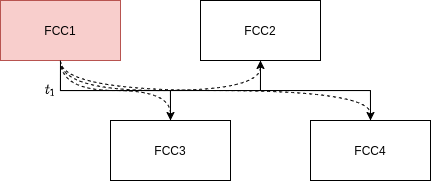
\includegraphics[width=0.6\textwidth]{img/byzantine_bus_1.png}
%     \caption{En este caso, la conexión tipo bus no permite el envío de información diferente a los demás miembros. La FCC1 envía el valor $t_1$ y todos sus pares reciben el mismo valor.}
%     \label{fig:byzantine_bus_1}    
% \end{figure}

% Como contrapartida, debido a que los nodos comparten canal de comunicación, estos deben tomar turnos para enviar la información a sus pares. De otra forma, habría una colisión en el bus y la información nunca llegaría a su destino. Sumado a esto, el bus se convierte en un punto singular de falla, ya que es posible que un problema en el bus deje a los nodos incomunicados.

%{\Large \textbf{{\color{red} ACÁ AGREGAR EJEMPLOS DE USO DE DOBLE BUS. POR EJEMPLO LOS AUTOS CON DOBLE CAN O DOBLE FLEX RAY, EL PAPER QUE USA DOBLE TIME TRIGGERED BUS, ETC}}}

% \subsubsection{Consenso}

% Al igual que como se hizo en la sección \ref{sec:consenso_TMR}, se analiza el problema del consenso para la arquitectura propuesta en esta sección. El ejemplo que se presentó anteriormente fue el necesario para lograr una sincronización entre las FCCs y se mostró que el enviar información distinta a cada computadora de vuelo, puede romper el sincronismo muy fácilmente.

% Para el caso en el que se utiliza un bus de comunicación, como se mencionó, las FCCs deben tomar turnos para utilizar el medio físico. En las próximas secciones se explicará cómo se puede lograr esto, aquí se asume que las FCCs respetan sus turnos para utilizar el medio físico compartido. En la figura \ref{fig:byzantine_bus_2}, la FCC1 accede al medio y envía su valor de \textit{timestamp}. Las demás FCCs reciben el mismo valor, por estar conectadas al mismo bus de comunicación. Luego, las FCC2 y 3 repiten esto mismo. En la figura \ref{fig:byzantine_bus_3} se muestra que todas tienen la misma información respecto de sus pares. Luego por ejemplo, si calculan un promedio, llegarán al mismo resultado y se sincronizarán correctamente.

% \begin{figure}[H]
%     \centering
%     \begin{subfigure}[b]{0.34\textwidth}
%         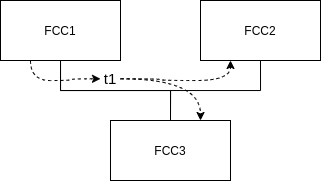
\includegraphics[width=\textwidth]{img/byzantine_bus_2.png}
%         \caption{La FCC1 envía su \textit{timestamp} hacia las demás.}
%         \label{fig:byzantine_bus_2}
%     \end{subfigure}\hfill
%     \begin{subfigure}[b]{0.49\textwidth}
%         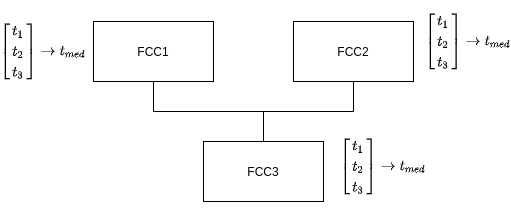
\includegraphics[width=\textwidth]{img/byzantine_bus_3.png}
%         \caption{Luego de finalizar los intercambios, todas las FCCs llegan al mismo resultado de \textit{timestamp} para sincronizarse.}
%         \label{fig:byzantine_bus_3}
%     \end{subfigure}
%     \caption{Debido a la existencia del bus, las FCCs no pueden mentir acerca de su \textit{timestamp}. Luego, todas llegan a un consenso de manera casi trivial.}
%     \label{}
% \end{figure}

% A partir de este análisis, se puede ver que para el caso de un sistema de tiempo real con un único bus de comunicaciones, el problema del consenso es mucho más sencillo que lo que se muestra en \textit{The Byzantine Generals Problem}. De todas maneras, lo que se presenta aquí es un primer análisis, ya que se ha asumido que no hay colisiones en el bus y que los nodos se encuentran sincronizados.

